\documentclass{article}
\usepackage{CJKutf8}
\usepackage[utf8]{inputenc}

\usepackage[nonatbib,final]{sty/neurips_2024}
\usepackage{sty/mymath}
\usepackage[utf8]{inputenc}
\usepackage[T1]{fontenc}
\usepackage{hyperref}
\usepackage{url}
\usepackage[
  style=alphabetic,
  backend=biber,
  maxalphanames=3,
  maxbibnames=20,
  maxcitenames=3,
  giveninits=true,
  doi=false,
  url=true,
  backref=true,
]{biblatex}
\usepackage{hyperref}
\hypersetup{
  colorlinks=true,
  linkcolor=blue,
  filecolor=magenta,
  urlcolor=cyan,
  citecolor=purple
}
\addbibresource{references.bib}
\usepackage{amsfonts}
\usepackage{amsmath}
 \usepackage{amsthm}
\usepackage{amssymb}
\usepackage{mathrsfs}
\usepackage{bm}
\usepackage{nicefrac}
\usepackage{xfrac}
\usepackage{subdepth}
\usepackage{array}
\usepackage{booktabs}
\usepackage{etoolbox}
\usepackage{microtype}
\usepackage[nameinlink,capitalise]{cleveref}
\usepackage[font=small,labelfont=bf]{caption}
\usepackage[format=hang]{subcaption}
\usepackage{graphicx}
\usepackage[export]{adjustbox}
\usepackage{color}
\usepackage{xcolor}
\usepackage{wrapfig}
\usepackage{multirow}
\usepackage{ifthen}
\usepackage{sidecap}
\crefname{lemma}{lemma}{lemmas}
\Crefname{lemma}{Lemma}{Lemmas}
\newcommand{\cf}{\textit{cf.}~}
\newcommand{\eg}{\textit{e.g.},~}
\newcommand{\ie}{\textit{i.e.},~}
\newcommand{\vs}{\textit{vs.}~}
\newcommand{\red}{\color{red}}
\newcommand{\blue}{\color{blue}}
\newcommand{\nb}[1]{{\sf\blue[#1]}}
\newcommand{\nbr}[1]{{\sf\red[#1]}}
\usepackage{marginnote}
\newcommand{\ignore}[1]{}
\newcommand{\todocite}[0]{{(\color{red}{citation needed}}) }
\definecolor{electric-purple}{RGB}{191, 0, 255}
\newcommand{\erin}[1]{{\sf\color{electric-purple}[Erin: #1]}}
\definecolor{kelly-green}{RGB}{45, 179, 0}
\newcommand{\forandrew}[1]{\marginnote{\tiny\textsf{\color{kelly-green}[#1]}}}
\newcommand{\andrew}[1]{{\sf\color{blue}[Andrew: #1]}}
\newcommand{\forleon}[1]{\marginnote{\tiny\textsf{\color{red}[#1]}}}
\renewcommand{\nb}[1]{}
\renewcommand{\nbr}[1]{}
\renewcommand{\erin}[1]{}
\title{
  神经感受野中局部化的非线性动力学
}
\author{
	Leon Lufkin \\
	Yale University \\
	\texttt{leon.lufkin@yale.edu} \\
    	\And
	Andrew Saxe \\
	Gatsby Unit \& SWC, UCL \\
	\texttt{a.saxe@ucl.ac.uk} \\
	\And
	Erin Grant \\
	Gatsby Unit \& SWC, UCL \\
	\texttt{erin.grant@ucl.ac.uk}
}
\usepackage{tcolorbox}
\usepackage{enumitem}
\tcbuselibrary{theorems, breakable, skins}
\tcbset{
  assumption-box/.style={
    enhanced,
    colback=white, colframe=black,
    colbacktitle=white, coltitle=black,
    boxed title style={size=small,colframe=white},
    boxrule=0.3mm,
    rounded corners,
    before upper={\parindent0pt},
    separator sign none,
    attach boxed title to top center={yshift=-3mm},
    before=\vspace{0pt},
    after=\vspace{5pt},
  }
}
\newtcbtheorem[no counter]{model}{}{
  assumption-box,
  before upper={
    \setlist[enumerate]{
      leftmargin=*,
      label=(M\arabic*),
      ref=M\thetcbcounter\arabic*,
    }
  },
}{prop}
\newtcbtheorem[no counter]{stimulus}{}{
  assumption-box,
  before upper={
    \setlist[enumerate]{
      leftmargin=*,
      label=(S\arabic*),
      ref=S\thetcbcounter\arabic*,
    }
  },
}{prop}
\newtcbtheorem[no counter]{analysis}{}{
  assumption-box,
  before upper={
    \setlist[enumerate]{
      leftmargin=*,
      label=(A\arabic*),
      ref=A\thetcbcounter\arabic*,
    }
  },
}{assumption}
\begin{document}
\begin{CJK*}{UTF8}{gbsn}

\maketitle

\begin{abstract}
  局部感受野——对输入的某些连续时空特征具有选择性的神经元——存在于哺乳动物大脑的早期感觉区域。优化显式稀疏性或独立性标准的无监督学习算法复制了这些局部感受野的特征,但未能直接解释在没有高效编码的情况下,如何通过学习实现局部化,正如在深度神经网络的早期层中发生的那样,也可能在生物系统的早期感觉区域中发生。我们考虑了一种替代模型,在该模型中,局部感受野在没有显式自上而下效率约束的情况下出现——一个基于自然图像结构启发的数据模型训练的前馈神经网络。先前的研究确定了非高斯统计对局部化的重要性,但对于推动动态涌现的机制仍然存在未解之谜。我们通过推导单个非线性神经元的有效学习动力学来解决这些问题,精确说明输入数据的高阶统计特性如何驱动涌现的局部化,并证明这些有效动力学的预测可以扩展到多神经元设置。我们的分析为局部化的普遍性提供了一种替代解释,认为局部化是神经电路中学习的非线性动力学的结果。\smash{\footnotemark}\footnotetext{
实验和图形的复现代码请见
\url{https://github.com/leonlufkin/localization}.
}

\end{abstract}

\section{引言}
\label{sec:introduction}

动物神经系统中外周反应的一个显著特征是 \emph{局部化}——也就是说,简单细胞神经元的线性感受野通常只对远小于其整个输入域的连续区域作出反应。
在视觉系统中,视网膜神经节细胞近似于对中心-周边区域的局部滤波器,这些滤波器铺满输入空间~\parencite{dacey2000center,doi2012efficient,knudsen1978space};
而在下游的初级视觉皮层中,简单细胞具有对空间频率和方向选择性的局部滤波器~\parencite{hubel1959receptive,hubel1968receptive,rolls1995sparseness,niell2008highly,willmore2011sparse,ringach2002orientation,ringach2002spatial}。
在初级躯体感觉皮层中,神经元对皮肤上受限区域的刺激产生反应~\parencite{crochet2011synaptic};
在初级听觉皮层中,时空感受野通常在时间和频率域中都是局部化的~\parencite{deweese2003binary,hromadka2008sparse};
参见 \cref{fig:sim-real-gabors}(左)。

相比之下,人工学习系统并不总是学习出局部化的滤波器。
主成分分析倾向于拟合跨越整个输入信号的权重,未加正则化的自编码神经网络架构和受限玻尔兹曼机也有类似表现~\parencite{saxe2011unsupervised}。
这一差异促使人们寻求能够从自然刺激中学习出局部感受野的人工学习模型,其中最具代表性的是稀疏编码~\parencite{olshausen1996emergence,olshausen1997sparse} 和独立成分分析~\parencite[ICA;~][]{bell1997independent,vanhateren1998independent}。
稀疏编码、ICA 及其他从自然数据中产生局部感受野的压缩方法采用的是自上而下的方式——它们通过优化显式的稀疏性准则,或在关键参数条件下需要稀疏性的独立性准则,从而找到输入信号的高效表示~\cite{field1999wavelets,saxe2011unsupervised}。

尽管稀疏性作为局部化的潜在统一解释具有吸引力,但局部化也会自然地出现在训练用于分类任务的网络中,即使这些网络并未显式使用稀疏性正则项~\parencite{krizhevsky2012imagenet,zeiler2013visualizing,yosinski2015understanding,sengupta2018manifoldtiling};
参见 \cref{fig:sim-real-gabors}(中)中的一个示例。
\textcite{ingrosso2022data} 提炼了此类涌现性局部化的示例,并展示了在简单前馈神经网络中,训练数据模型具有近似自然视觉输入特性的前提下,局部感受野会自然涌现出来,具体包括:
局部结构(非共址维度的统计独立性)以及非高斯性(高阶累积量非零)。
在模拟中,\textcite{ingrosso2022data} 将局部化的动态涌现与输入的高阶统计量调谐增强联系起来,并表明在这种设置下,甚至单个神经元也足以学习出局部感受野。

在本研究中,我们在 \textcite{ingrosso2022data} 的成果基础上进一步探究,旨在描述在该最小设置中局部感受野涌现背后的机制。
驱动局部化的高阶输入统计特性难以用现有依赖高斯性假设的分析工具进行研究~\parencite{goldt2020modelling}。
通过将学习过程划分为两个阶段,我们能够推导出在理想化自然数据驱动下,单个神经元模型在早期时间段的有效学习动力学方程。
我们的解析模型对驱动涌现的高阶统计特性给出了简洁的描述,
并通过多神经元模拟验证了该模型的正面与负面预测;参见 \cref{fig:sim-real-gabors}(右)。
这些发现提出了一种解释早期神经响应中普遍存在的局部化现象的替代路径,即源于神经回路中学习的非线性动态与具有高阶统计结构的自然数据之间的相互作用,
而非源于显式的效率准则。

\newcommand{\sampleheight}{42pt}
\newcommand{\covheight}{46pt}
\newcommand{\marginalheight}{50pt}
\setlength{\tabcolsep}{4pt}
\begin{figure}[t]
  \centering
  \hspace{-1.2em}
  \scalebox{0.9}{
  \begin{centering}
    \begin{tabular}{p{51pt}
      @{\hspace{10pt}}m{2pt}l
      @{\hspace{5pt}}l
      @{\hspace{10pt}}m{2pt}l
      @{\hspace{10pt}}m{2pt}l}
        \raisebox{18pt}{\small$\texttt{Ising}$} &
        \raisebox{34pt}{\rotatebox{90}{\tiny input value}} &
        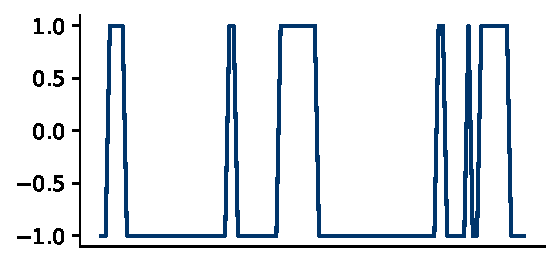
\includegraphics[height=\sampleheight]{figures/task/samples_long/ising.pdf} &
        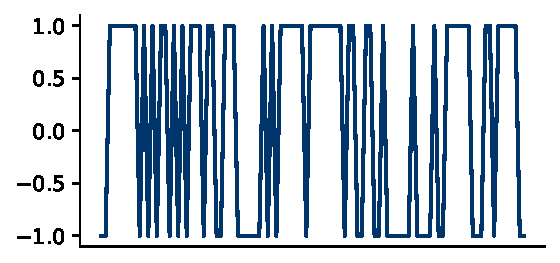
\includegraphics[height=\sampleheight]{figures/task/samples_short/ising.pdf} &
        \raisebox{38pt}{\rotatebox{90}{\tiny input dimension}} &
        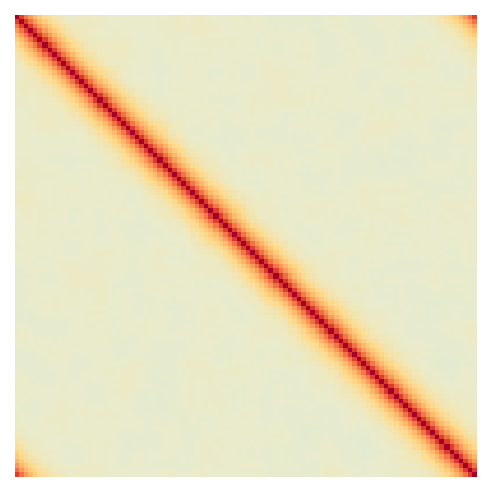
\includegraphics[height=\covheight]{figures/task/cov/ising.pdf} &
        \raisebox{40pt}{\rotatebox{90}{\tiny $p(X_i)$}} &
        \raisebox{-4pt}{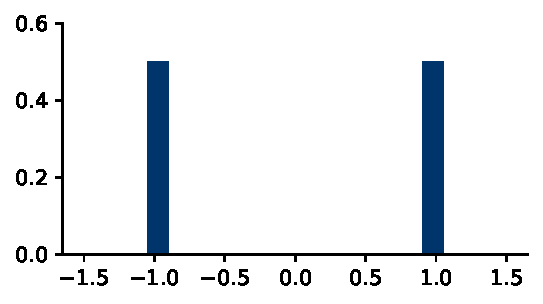
\includegraphics[height=\marginalheight]{figures/task/marginal/ising.pdf}} \\
        \noalign{\vskip -36pt}
        \raisebox{18pt}{\small$\texttt{NLGP}(0.01)$} &
        \raisebox{34pt}{\rotatebox{90}{\tiny input value}} &
        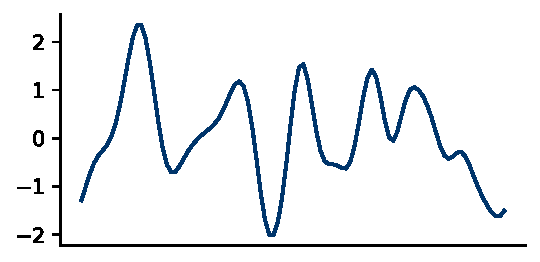
\includegraphics[height=\sampleheight]{figures/task/samples_long/gaussian.pdf} &
        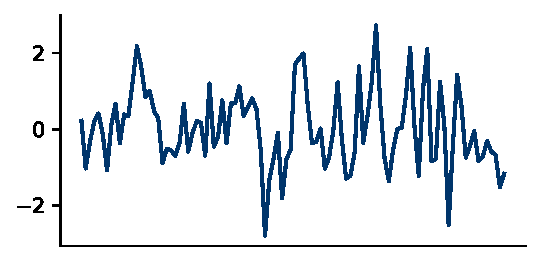
\includegraphics[height=\sampleheight]{figures/task/samples_short/gaussian.pdf} &
        \raisebox{38pt}{\rotatebox{90}{\tiny input dimension}} &
        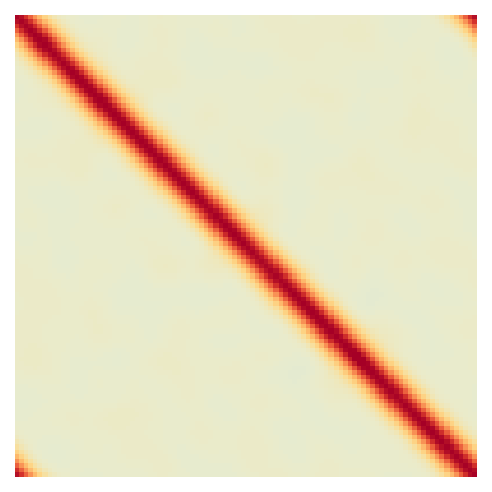
\includegraphics[height=\covheight]{figures/task/cov/gaussian.pdf} &
        \raisebox{40pt}{\rotatebox{90}{\tiny $p(X_i)$}} &
        \raisebox{-4pt}{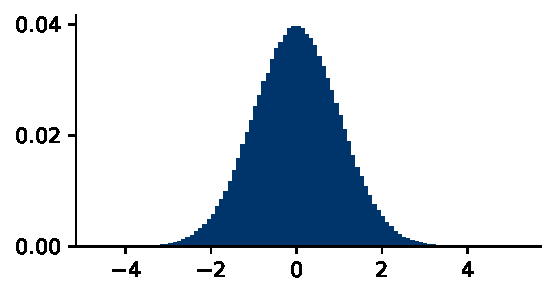
\includegraphics[height=\marginalheight]{figures/task/marginal/gaussian.pdf}} \\
        \noalign{\vskip -36pt}
        \raisebox{18pt}{\small $\texttt{Kur}(5)$} &
        \raisebox{34pt}{\rotatebox{90}{\tiny input value}} &
        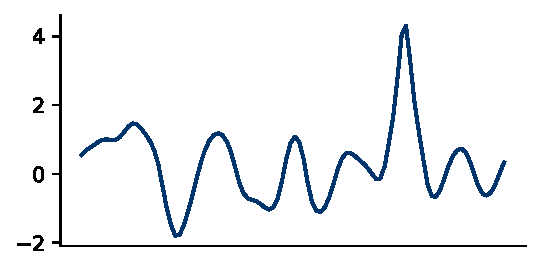
\includegraphics[height=\sampleheight]{figures/task/samples_long/alg5.pdf} &
        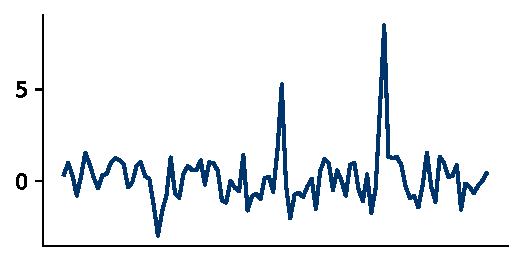
\includegraphics[height=\sampleheight]{figures/task/samples_short/alg5.pdf} &
        \raisebox{38pt}{\rotatebox{90}{\tiny input dimension}} &
        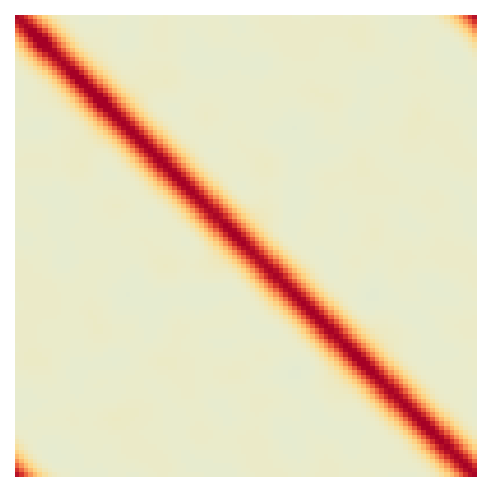
\includegraphics[height=\covheight]{figures/task/cov/alg5.pdf} &
        \raisebox{40pt}{\rotatebox{90}{\tiny $p(X_i)$}} &
        \raisebox{-4pt}{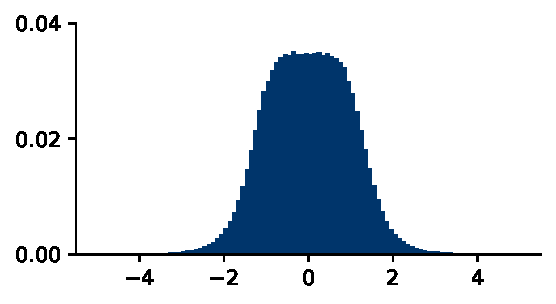
\includegraphics[height=\marginalheight]{figures/task/marginal/alg5.pdf}} \\
        \noalign{\vskip -37pt}
        &&
        \hspace{25pt}\tiny input dimension &
        \hspace{25pt}\tiny input dimension & &
        \hspace{3pt}\tiny input dimension & &
        \hspace{37pt}\tiny input value \\
  \end{tabular}
  \end{centering}
  }
  \caption{
    从左到右:
    长尺度和短尺度样本 $\mathbf{x}$,
    单一尺度的协方差 $\Sigma$,
    以及数据模型的边缘分布 $p(X_i)$,如 \cref{sec:task} 所述:
    Ising 模型(左、右样本分别为 $J=1.2, 0.3$),
    非线性高斯过程~\parencite[NLGP;~][]{ingrosso2022data},
    以及可控峰度模型 \texttt{Kur}
    (左、右样本分别为 $\xi=5, 1$)。
    \emph{
    每个模型生成的样本以零为中心,且其协方差可以被约束为相似,
    但具有不同的高阶统计量,从维度方向的边缘分布中可以看出这一点。
    }
}
  \label{fig:task}
  \vspace{-10pt}
\end{figure}

\section{Modeling approach}
\label{sec:prelims}

We extend the setting of \textcite{ingrosso2022data},
a minimal example of a neural network that learns localized receptive fields 
from idealized naturalistic data.
We analyze the dynamics of learning in this setting in \cref{sec:theory}
and validate our analytical model with simulations in \cref{sec:experiments}.

\subsection{Neural network architecture and learning algorithm}
\label{sec:model}

We consider a two-layer feedforward neural network with nonlinear activation and scalar output.
While simple, this architecture is highly expressive, capable of approximating arbitrary 
integrable univariate functions with appropriate scaling~\parencite{barron1993universal, pinkus1999approximation},
and exhibits rich feature learning dynamics that underlie the performance of models at scale~\parencite{woodworth2020kernel},
making this architecture the ongoing subject of theoretical neural network analyses~\parencite{mei2018mean, goldt2019dynamics, veiga2022phase}.
We denote a two-layer network with $N$-dimensional input, $M$ hidden units, and one-dimensional scalar output as
\newcounter{modelenumi}
\begin{model}{\textbf{Model 1} (\emph{many-neuron architecture}).}{}
\begin{enumerate}[series=modelenumi]
  \item \label{item:many-neuron-model} 
    \makebox[\linewidth - 2.5em]{
      $\hat{y}(\mathbf{x}) = b^{(2)} + \sum_{m=1}^M w_m^{(2)} 
      \sigma\left(b_m^{(1)} + \langle \mathbf{w}_m^{(1)}, \mathbf{x} \rangle \right)$
    }
\end{enumerate}
\end{model}
where $\sigma : \R \to \R$ is a pointwise nonlinearity such as the rectified linear unit (ReLU) or sigmoid function,
$\mathbf{w}_m^{(1)} \in \R^N$ and $w_m^{(2)} \in \R$ are learnable weights, 
$b_m^{(1)}, b^{(2)} \in \R$ are learnable bias terms, and
$\langle \cdot, \cdot \rangle$ denotes the standard Euclidean inner (dot) product on $\R^N$.
When the second-layer parameters are fixed, this model is known as a \emph{soft-committee machine}~\parencite[SCM;][]{saad1995line},
which~\parencite{ingrosso2022data} notes learns less noisy receptive fields but exhibits similar localization behavior.
The many-neuron architecture in \labelcref{item:many-neuron-model} is the focus of our \textbf{simulations}~(\cref{sec:experiments}), but the dynamics of this model 
are too complex to analyze directly, even for the idealized naturalistic data model considered here.
In order to derive \textbf{analytical} results~(\cref{sec:theory}), we consider the simplest neural network exhibiting the desired localization phenomenon, a single hidden neuron without bias and with rectified linear unit activation, written as
\begin{model}{\textbf{Model 2} (\emph{single-neuron architecture}).}{}
\begin{enumerate}[resume*=modelenumi]
  \item \label{item:single-neuron-model} 
    \makebox[\linewidth - 2.5em]{
      $\hat{y}(\mathbf{x}) = 
      \operatorname{ReLU}\left(\langle \mathbf{w}, \mathbf{x} \rangle \right)$
    }
\end{enumerate}
\end{model}
where $\operatorname{ReLU}(x) = \max(x,0)$, applied pointwise to vectorial input.
As \textcite{ingrosso2022data} demonstrate, the localized receptive fields learned by the 
many- and single-neuron models defined in \labelcref{item:many-neuron-model,item:single-neuron-model} are qualitatively similar up to spatial translation, 
which permits us to generalize insights from analyzing the learning dynamics of the single-neuron~\labelcref{item:single-neuron-model} to the many-neuron~\labelcref{item:many-neuron-model}.
For simulations, we initialize the weights and biases
as independent draws from an isotropic Gaussian distribution with scaled variance,
and train with batch gradient descent with a fixed learning rate on the mean-squared error
(MSE) evaluated on input-output pairs from the task; see \cref{sec:task} for task sampling procedures.

\subsection{Stimulus properties}
\label{sec:input}

The data model of \textcite{ingrosso2022data} 
can be shown to satisfy three conditions that enable the analysis we give in \cref{sec:theory}.
We consider several other data models that share the below properties but differ in generative mechanism
in order to probe the effect of these properties on localization.
In particular, we consider data $\mathbf{X}$ sampled from distributions $p$ on $\R^N$ satisfying the following:
\newcounter{propenumi}
\begin{stimulus}{\textbf{Stimulus properties 1--3} (\emph{idealization of natural images}).}{}
\begin{enumerate}[series=propenumi]
  \item \label{item:weak-dependence} (Positional) weak dependence: for any fixed $\rho \in (0,1)$, as $N \to \infty$,
    $$\alpha(N) \triangleq \sup_{A \subseteq \R, B \subseteq \R^{(1-\rho) N}} |\PR(X_1 \in A, X_{> \rho N} \in B) - \PR(X_1 \in A) \PR(X_{> \rho N} \in B)| \to 0~,$$
  \item \label{item:translation-invariance} Translation invariance: $p(\mathbf{X} = \mathbf{x}) = p(\mathbf{X} = \mathcal{S} \mathbf{x})$ for all $\mathbf{x} \in \R^N$, where $\mathcal{S}$ is the circular shift operator, and
  \item \label{item:sign-symmetry} Sign symmetry: $p(\mathbf{X} = \mathbf{x}) = p(\mathbf{X} = -\mathbf{x})$ for all $\mathbf{x} \in \R^N$.
\end{enumerate}
\end{stimulus}
Properties~\labelcref{item:weak-dependence,item:translation-invariance}
are defining characteristics of natural image data~\parencite{hyvarinen2009natural}.
Property~\labelcref{item:sign-symmetry}
can also be seen to hold for natural images after centering
and is convenient analytically
because it implies that $\E[\mathbf{X}] = 0$.
Property~\labelcref{item:weak-dependence} assumes that $p$ is implicitly parameterized by $N$
in order to state that the statistical dependence between entries of $\mathbf{X}$ vanishes 
as their separation increases.\smash{\footnotemark}\footnotetext{
  The weak dependence condition in \labelcref{item:weak-dependence} is based on strong $\alpha$-mixing, a notion first introduced by \cite{rosenblatt1956central} 
  to obtain a generalization of the central limit theorem, which we employ later on.
  We choose $\alpha$-mixing because it is easy to interpret and verify,
  but alternative definitions of weak dependence \parencite[\eg][]{bardet2008dependent} can be substituted.
}

We denote the covariance of $\mathbf{X}$ by $\Sigma \triangleq \operatorname{Cov}[\mathbf{X}]$,
the square of principal-diagonal entries (the variance of each entry of $\mathbf{X}$) by $\sigma^2$, 
and the $i$-th row by $\sigma_i$.
Weak dependence (\labelcref{item:weak-dependence}) implies that entries far from the principal diagonal of $\Sigma$ will be 0, while translation-invariance (\labelcref{item:translation-invariance}) implies that $\Sigma$ is circulant (\ie entries along each diagonal are equal) and thus identifiable by a single row; see \cref{fig:task} (center).

\subsection{Lengthscale discrimination task}
\label{sec:task}

\textcite{ingrosso2022data} develop a minimal task for which localization emerges in a feedforward neural network: binary discrimination between inputs from two distributions that differ in the lengthscale of the correlations between their entries.
This lengthscale discrimination task can be seen as a pretext task for self-supervised learning~\parencite{kolesnikov2019revisiting,chen2020simple} of representations~\parencite[\cf~unsupervised:][]{olshausen1996emergence,bell1997independent}.
More precisely, we generate data $(\mathbf{X},Y)$ for supervised training according to
\begin{align} \label{eq:task}
    \mathbf{X} \mid Y = y \sim p(\mathbf{X};\Sigma_y)~,
\end{align}
where $p$ is to be defined, $\Sigma_y$ are distinct covariance matrices for each $y$, and we sample $Y$ uniformly among a set of increasing \emph{lengthscale correlation classes} $y \in \{0,1,\ldots\}$, which correspond to the strength of correlation between distant positions.
For instance, in the case of two classes ($y = 0, 1$), we take $\Sigma_0$ to be closer to $\sigma^2 \mathbb{I}_N$ than $\Sigma_1$, where $\mathbb{I}_N$ is the $N \times N$ identity matrix and $\sigma$ is a fixed value.
This construction isolates, via distinct covariance matrices per class, the second-order statistics, which we will see below enter into the learning dynamics separately from other properties of $p(\mathbf{X})$, including, most critically, the implied marginal distributions, $p(X_i)$.

\paragraph{\texttt{Ising}.}\hspace{-2pt}
The first distribution we consider is the one-dimensional Ising model.
It is of interest as a distribution that satisfies \labelcref{item:weak-dependence,item:translation-invariance,item:sign-symmetry} with marginals $p(X_i)$ with extreme support on $\{ \pm 1 \}$,
making it the distribution that promotes localization most strongly, as we will see in \cref{sec:theory}.
In the absence of an external field, the Ising distribution is
\begin{equation}
    p_\text{\texttt{Ising}}(\mathbf{X}=\mathbf{x})
    = p_\text{\texttt{Ising}}(X_1=x_1,\ldots,X_N=x_N) = e^{ -\sum_{i=1}^{N} J x_i x_{i+1} } / \mathcal{Z},
\end{equation}
where $J$ is a chosen pairwise interaction strength, $\mathcal{Z}$ is the normalizing constant, and we enforce a periodic boundary constraint via $x_{N+1} \equiv x_1$.
As $J$ increases, the lengthscale of the correlations in $\mathbf{X}$ also increases.
For simulations, we sample from $p_\texttt{Ising}$ using a Gibbs sampler~\parencite{geman1984stochastic}.
Discrimination tasks in the simulations in 
\cref{sec:experiments}
use $J_1=0.7$ (for $y=1$) and $J_0=0.3$ (for $y=0$).

\newcommand{\sampleheight}{42pt}
\newcommand{\covheight}{46pt}
\newcommand{\marginalheight}{50pt}
\setlength{\tabcolsep}{4pt}
\begin{figure}[t]
  \centering
  \hspace{-1.2em}
  \scalebox{0.9}{
  \begin{centering}
    \begin{tabular}{p{51pt}
      @{\hspace{10pt}}m{2pt}l
      @{\hspace{5pt}}l
      @{\hspace{10pt}}m{2pt}l
      @{\hspace{10pt}}m{2pt}l}
        \raisebox{18pt}{\small$\texttt{Ising}$} &
        \raisebox{34pt}{\rotatebox{90}{\tiny input value}} &
        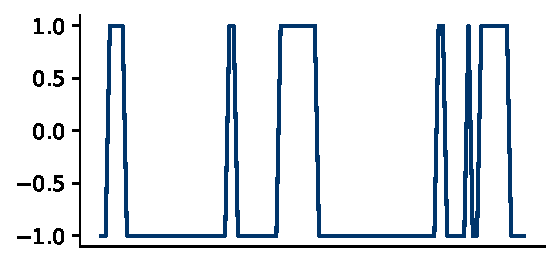
\includegraphics[height=\sampleheight]{figures/task/samples_long/ising.pdf} &
        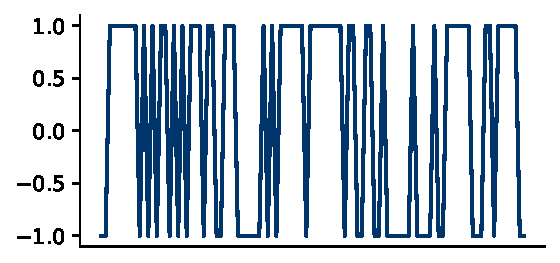
\includegraphics[height=\sampleheight]{figures/task/samples_short/ising.pdf} &
        \raisebox{38pt}{\rotatebox{90}{\tiny input dimension}} &
        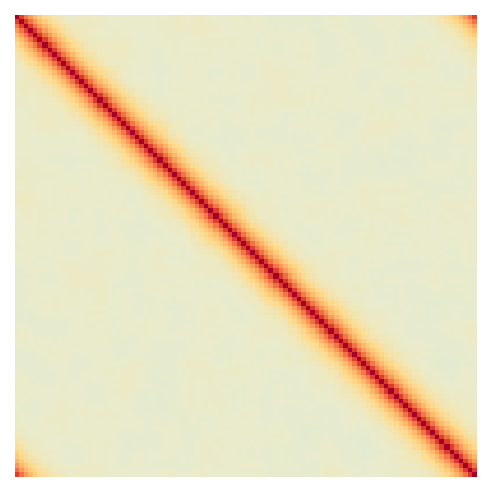
\includegraphics[height=\covheight]{figures/task/cov/ising.pdf} &
        \raisebox{40pt}{\rotatebox{90}{\tiny $p(X_i)$}} &
        \raisebox{-4pt}{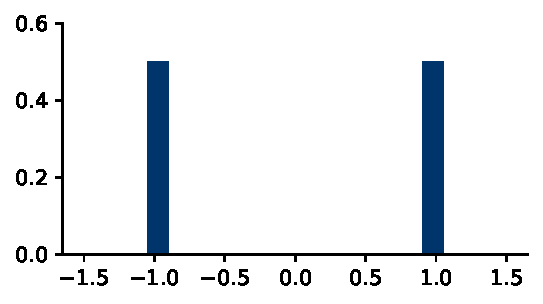
\includegraphics[height=\marginalheight]{figures/task/marginal/ising.pdf}} \\
        \noalign{\vskip -36pt}
        \raisebox{18pt}{\small$\texttt{NLGP}(0.01)$} &
        \raisebox{34pt}{\rotatebox{90}{\tiny input value}} &
        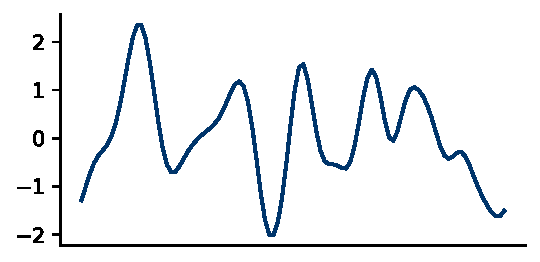
\includegraphics[height=\sampleheight]{figures/task/samples_long/gaussian.pdf} &
        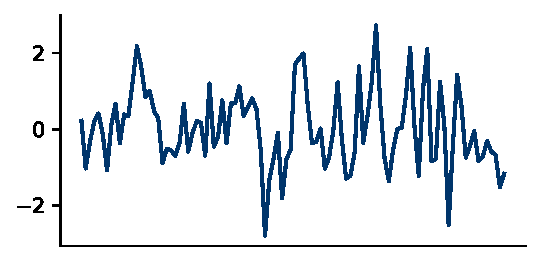
\includegraphics[height=\sampleheight]{figures/task/samples_short/gaussian.pdf} &
        \raisebox{38pt}{\rotatebox{90}{\tiny input dimension}} &
        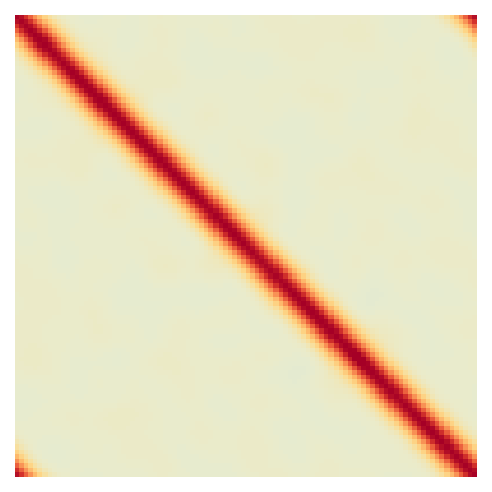
\includegraphics[height=\covheight]{figures/task/cov/gaussian.pdf} &
        \raisebox{40pt}{\rotatebox{90}{\tiny $p(X_i)$}} &
        \raisebox{-4pt}{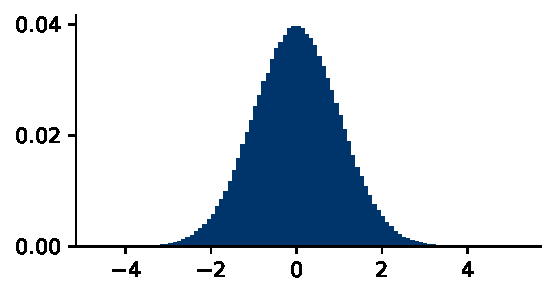
\includegraphics[height=\marginalheight]{figures/task/marginal/gaussian.pdf}} \\
        \noalign{\vskip -36pt}
        \raisebox{18pt}{\small $\texttt{Kur}(5)$} &
        \raisebox{34pt}{\rotatebox{90}{\tiny input value}} &
        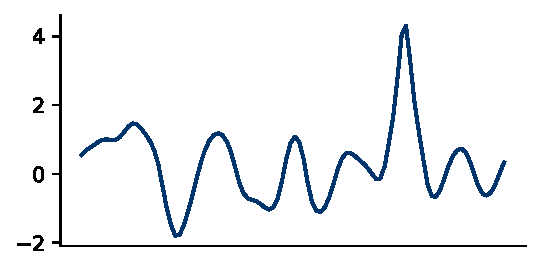
\includegraphics[height=\sampleheight]{figures/task/samples_long/alg5.pdf} &
        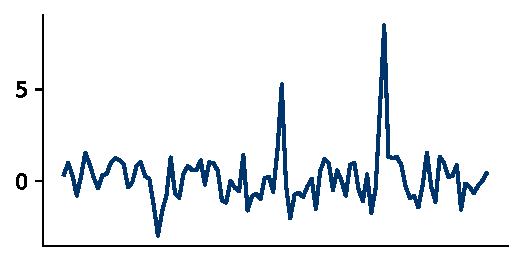
\includegraphics[height=\sampleheight]{figures/task/samples_short/alg5.pdf} &
        \raisebox{38pt}{\rotatebox{90}{\tiny input dimension}} &
        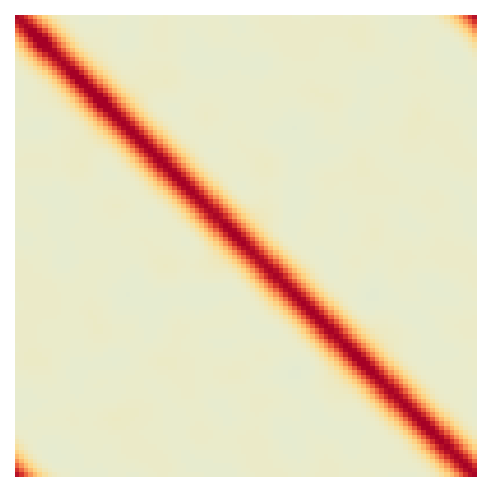
\includegraphics[height=\covheight]{figures/task/cov/alg5.pdf} &
        \raisebox{40pt}{\rotatebox{90}{\tiny $p(X_i)$}} &
        \raisebox{-4pt}{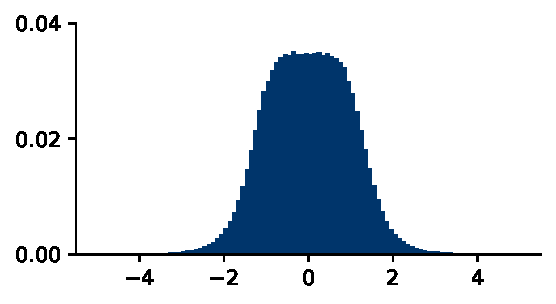
\includegraphics[height=\marginalheight]{figures/task/marginal/alg5.pdf}} \\
        \noalign{\vskip -37pt}
        &&
        \hspace{25pt}\tiny input dimension &
        \hspace{25pt}\tiny input dimension & &
        \hspace{3pt}\tiny input dimension & &
        \hspace{37pt}\tiny input value \\
  \end{tabular}
  \end{centering}
  }
  \caption{
    从左到右:
    长尺度和短尺度样本 $\mathbf{x}$,
    单一尺度的协方差 $\Sigma$,
    以及数据模型的边缘分布 $p(X_i)$,如 \cref{sec:task} 所述:
    Ising 模型(左、右样本分别为 $J=1.2, 0.3$),
    非线性高斯过程~\parencite[NLGP;~][]{ingrosso2022data},
    以及可控峰度模型 \texttt{Kur}
    (左、右样本分别为 $\xi=5, 1$)。
    \emph{
    每个模型生成的样本以零为中心,且其协方差可以被约束为相似,
    但具有不同的高阶统计量,从维度方向的边缘分布中可以看出这一点。
    }
}
  \label{fig:task}
  \vspace{-10pt}
\end{figure}


\paragraph{\texttt{NLGP}$(g)$.}\hspace{-2pt}
We also consider the data model used in \textcite{ingrosso2022data}, the nonlinear Gaussian process (NLGP), which enables one to interpolate between distributions that do and do not yield localization via a single parameter, $g$.
A sample $\mathbf{X} \mid Y = y$ from the NLGP is constructed by first sampling a Gaussian $\mathbf{Z} \mid Y = y \sim \NN(0, \tilde{\Sigma}_y)$ and then transforming it via
\begin{equation} \label{eq:nlgp}
    X_i \triangleq \operatorname{erf}(g Z_i) / \mathcal{Z}(g) \qquad 1 \leq i \leq N,
\end{equation}
where $\operatorname{erf}$ is the Gauss error function, $\mathcal{Z}$ is a normalization constant to ensure that the variances of $X_i$ and $Z_i$ are the same, and $\tilde{\Sigma}_y$ is a covariance matrix for $\mathbf{Z}$, where we use $(\tilde{\Sigma}_y)_{ij} = \exp(-(i-j)^2/\xi^2)$ for a lengthscale parameter $\xi$ \cite{ingrosso2022data}. 
If $g \approx 0$ (where localization is \emph{not} observed), $g Z_i$ will tend to lie in the linear regime of $\operatorname{erf}$, so $Z_i$ will be untransformed, \ie $\mathbf{X}$ is Gaussian.
However, as $g \to \infty$ (where localization \emph{is} observed), $g Z_i$ will tend to saturate $\operatorname{erf}$, so $X_i$ will have support on $\{ \pm 1 \}$.

\paragraph{\texttt{Kur}$(k)$.}\hspace{-2pt}
The final family we consider is chosen to give us flexibility over the kurtosis $\kappa$ of the marginals $p(X_i)$.
In the Ising model, the \emph{excess} kurtosis ($\kappa - 3$) of the marginals is fixed at $-2$, while in $\texttt{NLGP}(g)$, it varies from $-2$ to $0$.
This family allows us to vary the excess kurtosis from negative through positive values.
We sample $\mathbf{X} \mid Y = y$ from this family via inverse transform sampling to vary the marginals while enforcing dependence via Gaussian copulas.
More concretely, we sample $\mathbf{Z} \mid Y = y \sim \NN(0, \tilde{\Sigma}_y)$ and then transform it via
\begin{equation}
    X_i \triangleq f^{-1}( \Phi( Z_i / \tilde{\sigma} )) / \mathcal{Z}, \qquad 1 \leq i \leq N, \label{eq:alg}
\end{equation}
where $\tilde{\sigma}$ is the standard deviation of $Z_i$, $\Phi$ is the standard Gaussian cumulative distribution function (CDF), $f$ is the CDF of the desired marginal distribution for $X_i$, and $\mathcal{Z}$ is a normalization constant, which we compute numerically.
We define $\tilde{\Sigma}_y$ as for $\texttt{NLGP}$.
We choose $f$ to be the generalized \emph{algebraic sigmoid} function (see \cref{sec:algebraic-sigmoid})
for $k > 0$ to make use of its tractable inverse, simplifying the procedure in \cref{eq:alg}.
We denote the corresponding distribution by $\texttt{Kur}(k)$.
Though we are able to continuously vary excess kurtosis, we lack an explicit form; however, numerical computation shows that for $k \lessapprox 5.8$, excess kurtosis is positive, while for $k \gtrapprox 5.9$, it is negative.

\section{理论结果}
\label{sec:theory}

我们推导了\labelcref{item:single-neuron-model}中单神经元架构的定位动态的解析模型。
该结果建立了在性质~\labelcref{item:weak-dependence,item:translation-invariance,item:sign-symmetry}下实现定位的充要条件,适用于响应为二值的最简情形,\ie $y = 0,1$。
\cref{sec:experiments} 中展示了,在\labelcref{item:single-neuron-model}中的单神经元架构的定位条件,在经验上同样适用于\labelcref{item:many-neuron-model}中的多神经元架构。
此外,我们利用该模型推导出一个关于定位的负向预测,即尽管这些架构具有非高斯的统计特性——尤其是显著正的峰度——它们在椭圆分布上仍未能学习出局部化的感受野~\parencite[\cf 正峰度作为定位的目标函数或诊断工具,][]{hyvarinen2000independent,ingrosso2022data}。
\subsection{单神经元中定位动力学的分析模型}

先前的研究方法在\labelcref{item:many-neuron-model,item:single-neuron-model}的架构中研究了梯度流,假设预激活$\langle \mathbf{w}, \mathbf{X} \rangle$近似为高斯分布~\parencite{goldt2020modelling,gerace2020generalisation,goldt2022gaussian},但这一假设未能捕捉到通过神经网络传播的高阶统计量,这些统计量促进了定位现象~\cite{ingrosso2022data}。幸运的是,在\labelcref{item:weak-dependence,item:translation-invariance,item:sign-symmetry}中提出的理想化视觉输入设置允许我们进行一些简化。特别地,数据$\mathbf{X}$在\labelcref{item:translation-invariance}下的平移不变性以及\labelcref{item:single-neuron-model}中的架构允许我们使用每个输入维度$X_i$的边际分布,而不是$\mathbf{X}$的联合分布。

我们现在给出允许我们推导单神经元架构中定位动力学的分析模型的简化假设,即对所有$i \in \{1, \dots, N\}$,$\mathbf{X} \mid X_i$的两个假设,以及初始化时满足的权重的温和条件。具体来说,$\sigma_i^y$表示$\Sigma_y$的第$i$行:

\newcounter{assumenumi}
\begin{analysis}{\textbf{解析简化 1--3} (\emph{早期时间,极限动态})}{}
\begin{enumerate}[series=assumenumi]
  \item \label{item:mean-assumption} $\E[\mathbf{X} \mid X_i = x_i, Y = y] = x_i \sigma_i^y$,即条件均值与 $x_i$ 成线性关系。
  \item \label{item:covariance-assumption} $\text{Cov}[\mathbf{X} \mid X_i = x_i, Y = y] = \Sigma_y - \sigma_i^y \sigma_i^{y\top}$,即条件协方差在 $i$ 附近较小,但与 $x_i$ 的确切值无关。
  \item \label{item:lindeberg-condition} Lindeberg 条件对序列 $w_1 X_1, \ldots, w_N X_N \mid X_i = x_i$ 在 $N \to \infty$ 时对所有 $x_i$ 都成立。
\end{enumerate}
\end{analysis}

假设~\labelcref{item:mean-assumption,item:covariance-assumption,item:lindeberg-condition}的动机是,它们复制了边际分布$X_i$(稍后进一步讨论)的峰度,这对于两个重要且不同的极限情形至关重要,其中分别出现和不出现定位现象:当$\mathbf{X}$的支持集中在超立方体的顶点上$\{ \pm 1 \}^N$(对于任意$J$,\texttt{Ising}满足此条件),以及当$\mathbf{X}$是高斯分布时(对于$g \approx 0$的\texttt{NLGP}满足此条件)。

引理~\labelcref{lem:gradient_flow}中的梯度流也依赖于假设~\labelcref{item:lindeberg-condition},即Lindeberg条件对于序列$w_i X_i$成立,这确保了序列中的任何单一项$w_i X_i$不能占主导地位。如果这一条件成立,我们可以得出结论,$\langle \mathbf{w}, \mathbf{X} \rangle \mid X_i$近似为高斯分布。正如我们在\cref{subsec:pf_of_gradient_flow}中讨论的,这几乎总是对$\mathbf{w}$的高斯初始化成立,且对轻微偏离这一初始化的情况也成立,并且满足\textcite{ingrosso2022data}的设置。利用这一事实,我们得到了训练初期梯度流的显式形式,如引理~\labelcref{lem:gradient_flow}所述。

\begin{lemma} \label{lem:gradient_flow}
    在假设~\labelcref{item:mean-assumption,item:covariance-assumption} 下,
    单个ReLU神经元的梯度流在训练初期,假设$y = 0, 1$,使用MSE损失函数时的表达式为
    \begin{equation} \label{eq:gradient_flow_early}
      \frac{2}{\tau} \frac{\mathrm{d}\mathbf{w}}{\mathrm{d}t} = \varphi\left( \frac{\Sigma_1 \mathbf{w}}{\sqrt{\langle \Sigma_1 \mathbf{w}, \mathbf{w} \rangle}} \right) - ( \Sigma_0 + \Sigma_1 ) \mathbf{w} + o_N(1),
    \end{equation}
    其中$o_N(1)$在$N\to\infty$时消失,并且$\varphi : (-1,1) \to \R$ 定义为
    \begin{equation} \label{eq:varphi}
        \varphi(a) = \E_{X_1 \mid Y = 1}\left[ X_1 \operatorname{erf}\left( X_1 \operatorname{alg}^{-1}(a) / \sqrt{2} \right)
        \right]
    \end{equation}
    并且$\operatorname{alg}^{-1}(x) = x/\sqrt{1-x^2}$,是代数sigmoid函数$\operatorname{alg}(x) = x/\sqrt{1+x^2}$的逆函数。
\end{lemma}
引理~\labelcref{lem:gradient_flow}将高阶统计量的研究简化为边际分布$X_1$,由于平移不变性,所有边际分布具有相同的分布,因此我们可以不失一般性地讨论$X_1$。尽管引理~\labelcref{lem:gradient_flow}严格而言只在训练初期成立,且如果$\mathbf{w}$由于违反\labelcref{item:lindeberg-condition}而变得定位,则该引理会失效,但\cref{eq:gradient_flow_early}中的梯度流在足够长的时间内保持有效,足以检测到权重$\mathbf{w}$中的定位现象。特别地,数值积分\cref{eq:gradient_flow_early}会在$t \to \infty$时得到定位的权重$\mathbf{w}$。此外,\cref{eq:gradient_flow_early}中的最终权重峰值的位置与实际观察到的定位峰值位置非常接近;有关这一事实的经验验证,请参见\cref{sec:peak-prediction}。观察到的主要差异是,\cref{eq:gradient_flow_early}中的定位峰值比精确计算的峰值略为平缓;有关实验观测到的定位感受野与理论预测之间的比较,请参见\cref{fig:theory}。
\subsection{涌现局部化的必要和充分条件}
\label{subsec:localization_conditions}

要确定局部化出现的精确阈值,需要求解\cref{eq:gradient_flow_early},但对于一般的非线性微分方程,无法精确求解。\smash{\footnotemark}\footnotetext{
我们在\cref{sec:pde-limit}中讨论了一个面临类似难以处理的偏微分方程极限问题。
}
尽管如此,\cref{eq:gradient_flow_early}的形式表明局部化仅由第一项驱动。
实际上,第二项仅依赖于数据的二阶统计量,因此可以在从诱导局部化的分布变化到不诱导局部化的分布时保持固定。
其次,可以看出,\cref{eq:gradient_flow_early}中的第一项在$\mathbf{w}$缩放时不发生变化,而第二项则有所不同。
因此,\cref{eq:gradient_flow_early}中的第二项用于约束$\mathbf{w}$的\emph{尺度},与局部化不同,而第一项则主要关注$\mathbf{w}$的\emph{形状},因此与局部化相关。
这进一步推动了第一项的关注,因此我们将其称为\emph{放大器},并且它本身依赖于数据分布$p(\mathbf{X})$的性质,
作为研究局部化的重点。

\newcommand{\sampleheight}{42pt}
\newcommand{\covheight}{46pt}
\newcommand{\marginalheight}{50pt}
\setlength{\tabcolsep}{4pt}
\begin{figure}[t]
  \centering
  \hspace{-1.2em}
  \scalebox{0.9}{
  \begin{centering}
    \begin{tabular}{p{51pt}
      @{\hspace{10pt}}m{2pt}l
      @{\hspace{5pt}}l
      @{\hspace{10pt}}m{2pt}l
      @{\hspace{10pt}}m{2pt}l}
        \raisebox{18pt}{\small$\texttt{Ising}$} &
        \raisebox{34pt}{\rotatebox{90}{\tiny input value}} &
        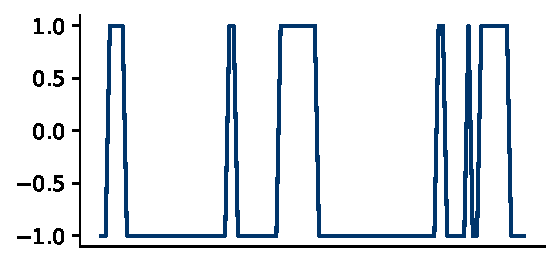
\includegraphics[height=\sampleheight]{figures/task/samples_long/ising.pdf} &
        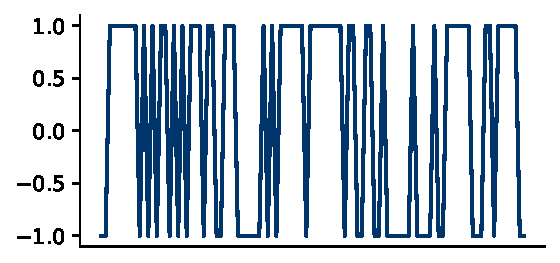
\includegraphics[height=\sampleheight]{figures/task/samples_short/ising.pdf} &
        \raisebox{38pt}{\rotatebox{90}{\tiny input dimension}} &
        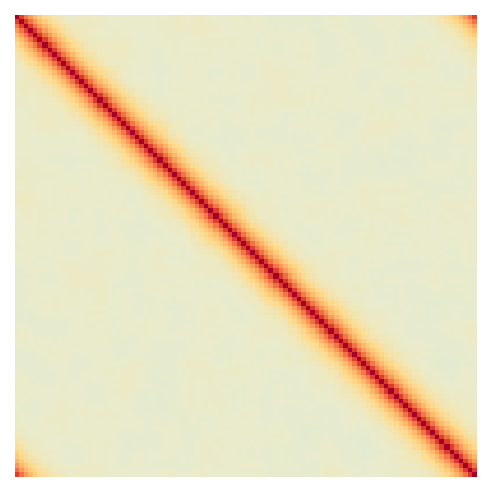
\includegraphics[height=\covheight]{figures/task/cov/ising.pdf} &
        \raisebox{40pt}{\rotatebox{90}{\tiny $p(X_i)$}} &
        \raisebox{-4pt}{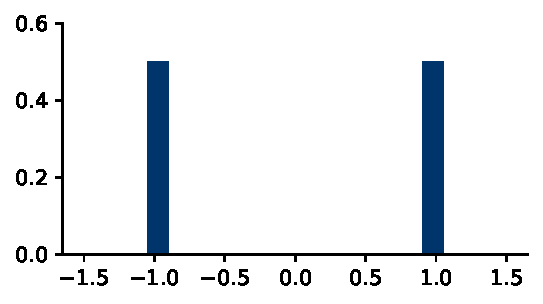
\includegraphics[height=\marginalheight]{figures/task/marginal/ising.pdf}} \\
        \noalign{\vskip -36pt}
        \raisebox{18pt}{\small$\texttt{NLGP}(0.01)$} &
        \raisebox{34pt}{\rotatebox{90}{\tiny input value}} &
        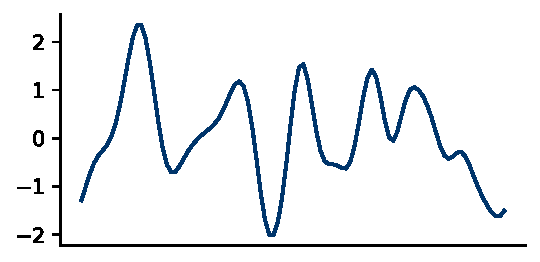
\includegraphics[height=\sampleheight]{figures/task/samples_long/gaussian.pdf} &
        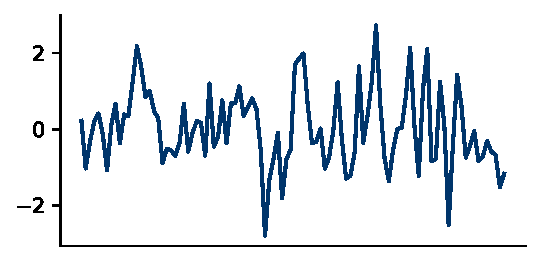
\includegraphics[height=\sampleheight]{figures/task/samples_short/gaussian.pdf} &
        \raisebox{38pt}{\rotatebox{90}{\tiny input dimension}} &
        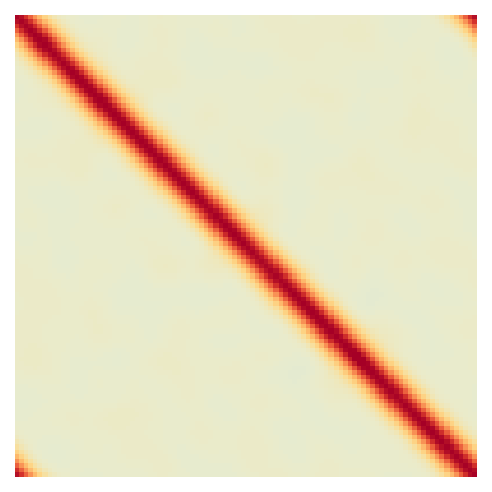
\includegraphics[height=\covheight]{figures/task/cov/gaussian.pdf} &
        \raisebox{40pt}{\rotatebox{90}{\tiny $p(X_i)$}} &
        \raisebox{-4pt}{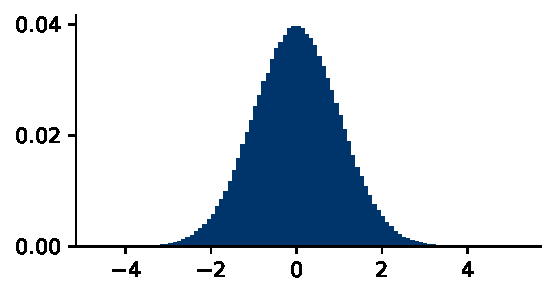
\includegraphics[height=\marginalheight]{figures/task/marginal/gaussian.pdf}} \\
        \noalign{\vskip -36pt}
        \raisebox{18pt}{\small $\texttt{Kur}(5)$} &
        \raisebox{34pt}{\rotatebox{90}{\tiny input value}} &
        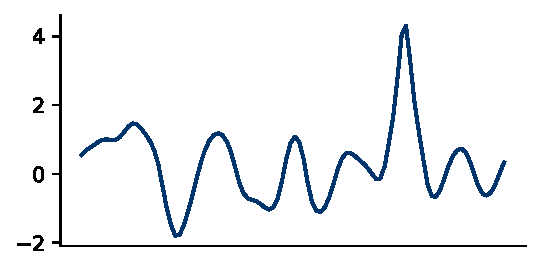
\includegraphics[height=\sampleheight]{figures/task/samples_long/alg5.pdf} &
        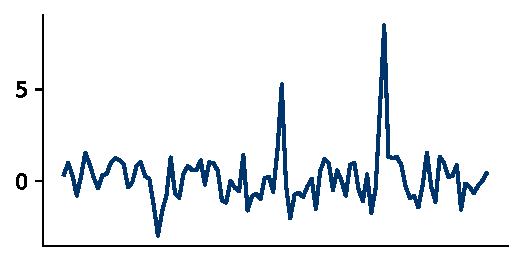
\includegraphics[height=\sampleheight]{figures/task/samples_short/alg5.pdf} &
        \raisebox{38pt}{\rotatebox{90}{\tiny input dimension}} &
        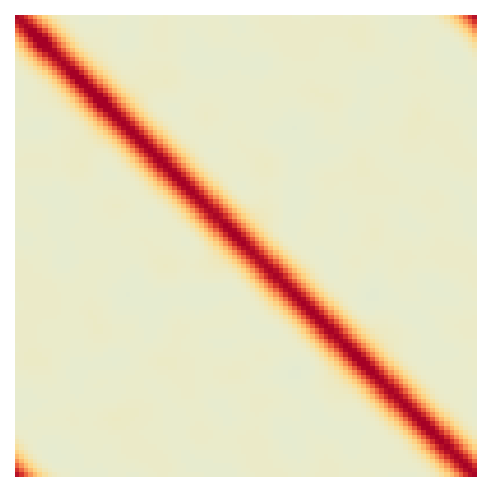
\includegraphics[height=\covheight]{figures/task/cov/alg5.pdf} &
        \raisebox{40pt}{\rotatebox{90}{\tiny $p(X_i)$}} &
        \raisebox{-4pt}{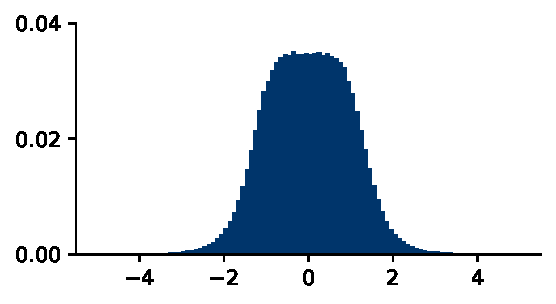
\includegraphics[height=\marginalheight]{figures/task/marginal/alg5.pdf}} \\
        \noalign{\vskip -37pt}
        &&
        \hspace{25pt}\tiny input dimension &
        \hspace{25pt}\tiny input dimension & &
        \hspace{3pt}\tiny input dimension & &
        \hspace{37pt}\tiny input value \\
  \end{tabular}
  \end{centering}
  }
  \caption{
    从左到右:
    长尺度和短尺度样本 $\mathbf{x}$,
    单一尺度的协方差 $\Sigma$,
    以及数据模型的边缘分布 $p(X_i)$,如 \cref{sec:task} 所述:
    Ising 模型(左、右样本分别为 $J=1.2, 0.3$),
    非线性高斯过程~\parencite[NLGP;~][]{ingrosso2022data},
    以及可控峰度模型 \texttt{Kur}
    (左、右样本分别为 $\xi=5, 1$)。
    \emph{
    每个模型生成的样本以零为中心,且其协方差可以被约束为相似,
    但具有不同的高阶统计量,从维度方向的边缘分布中可以看出这一点。
    }
}
  \label{fig:task}
  \vspace{-10pt}
\end{figure}


我们在\cref{sec:varphi-analysis}中对$\varphi$进行了分析,揭示了数据的边际分布在驱动局部化中的作用。
对于每个边际,$\varphi(a) \approx (\sqrt{2/\pi}) a$,当$a \approx 0$时成立。
对于较大的$a$,$\varphi$更强烈地依赖于数据分布,可能是超线性的(亚线性),即大于(小于)$(\sqrt{2/\pi}) a$。
超线性的$\varphi$鼓励在某些邻域中较大的$\mathbf{w}$条目增长得比较小的条目更快,从而产生局部化。
线性和亚线性的$\varphi$则相反,通过抑制$\mathbf{w}$中的邻域,鼓励振荡或平坦的权重。
然而,超线性和亚线性可能并不总是成立,因为$\varphi$可以在其定义域内同时存在(参见\cref{fig:theory},底行,黑线)。
作为一种近似方法,我们考虑了三阶泰勒展开(见\cref{fig:theory}第二列中的红线),这揭示了对于$\sigma^2 = 1$的典型设置,\emph{边际的负过度峰度导致超线性},而\emph{正过度峰度则导致亚线性};
见\cref{sec:varphi-analysis}。
这导致了以下主张,并通过我们在\cref{sec:experiments}中的模拟得到了验证:
\begin{claim} \label{thm:localization}
    对于足够大的 $N$,如果数据 $\mathbf{X} \in \R^N$ 满足条件 \labelcref{item:weak-dependence,item:translation-invariance,item:sign-symmetry} 并且其边际分布具有足够的 \emph{负}过度峰度,则模型~\labelcref{item:single-neuron-model} 将学习到局部化的感受野。
    相反,如果过度峰度足够 \emph{正},则不会。
\end{claim}

作为一个最小的正例,具有最负过度峰度的分布是对称的伯努利分布,峰度值为$-2$。
在我们的设置中,这对应于一个数据向量$\mathbf{X}$,其支持在超立方体的顶点上,$\{ \pm 1 \}^N$。
如上所述,可以从总协方差法则结合符号对称性看出,\labelcref{item:mean-assumption,item:covariance-assumption}完全成立。
请注意,$\varphi$对于所有此类分布是相同的,这使我们得出了\labelcref{thm:localization}的主张,即\emph{任何}满足条件\labelcref{item:weak-dependence,item:translation-invariance,item:sign-symmetry}的分布,其边际最大集中,将在~\labelcref{item:single-neuron-model}中引发局部化的感受野。
值得注意的是,这一主张包括了\textcite{ingrosso2022data}的极限情形,即$\texttt{NLGP}$中的$g\to\infty$。
它还包括了伊辛模型作为另一个例子,验证了对限制玻尔兹曼机的观察 \cite{harsh2020placecell},即伊辛数据在学习模型中引发局部化。
这些主张在\cref{fig:theory}中对单神经元模型进行了验证,并在\cref{sec:experiments}中的多神经元模型中得到了验证。
\subsection{案例研究:椭圆分布未能产生局部化}
\label{sub:elliptical}

如上所述,我们假设弱依赖性(\labelcref{item:weak-dependence})使我们能够专注于边缘分布如何控制局部化。
作为对这种假设的首次调查,我们考虑从椭圆分布中采样的数据 $\mathbf{X}$,其中弱依赖性可能不成立。
我们将椭圆分布的定义~\parencite{frahm2004generalized}专门化到我们的多类标签和符号对称性的设置:
\begin{definition}
    \label{def:elliptical}
    样本 $\mathbf{X} \in \R^N$ 满足 \emph{椭圆分布},如果我们可以写成
    $\mathbf{X} \mid Y = y \overset{(d)}{=} R_y \Lambda_y \mathbf{U}_y$
    其中 $R_y$ 是一个非负随机变量,$\Lambda_y \in \R^{N \times D}$ 满足 $\Lambda_y \Lambda_y^\top = \Sigma_y$,并且 $\mathbf{U}_y$ 与 $R_y$ 独立且在 $D$ 维球面上均匀分布。
\end{definition}

椭圆分布类是广泛的,仅要求密度的等高线是椭圆形的;多元高斯分布和Student-$t$分布就是例子。
因此,它们在非高斯性度量(包括峰度)上可以变化很大,同时保持足够的结构以便于分析。
命题 \labelcref{thm:elliptical} 表明,在单个ReLU神经元模型中,训练椭圆数据会\emph{防止}局部化。
\begin{proposition} \label{thm:elliptical}
  假设数据 $\mathbf{X}$ 是
  符号对称的 (\labelcref{item:sign-symmetry}),
  平移不变的 (\labelcref{item:translation-invariance}),
  并且服从椭圆分布,使得在 \cref{sec:task} 中的任务的均方误差(MSE)始终是有限的。
  如果 $\Sigma_0, \Sigma_1$ 满足它们的第 $i$ 个特征值比率 $\lambda_i(\Sigma_0) / \lambda_i(\Sigma_1)$ 仅在最多两个不同的 $i$ 处取特定值,则 \labelcref{item:single-neuron-model} 中权重的稳态是正弦波,即不局部化。
\end{proposition}

对于数字 $i$ 的条件,使得 $i$-th 特征值的比率相同,限制了在$\mathbf{w}$的稳态中可以非零的傅里叶分量的数量。
尽管这一要求较为晦涩,但在实践中似乎总是成立,因为即使是轻微的长度尺度相关性增加,也能显著改变$\Sigma_y$的谱。

这一命题令人惊讶,因为它揭示了预激活的峰度并不是解释局部化的合适指标。
考虑$N$维Student-$t$分布的例子,具有$\nu$自由度,$t_N(\nu)$。
如果 $\mathbf{X} \sim t_N(\nu)$,则 $\langle w, \mathbf{X} \rangle \sim t_1(\nu)$。
注意,$t_1(\nu)$的峰度是非零的,对于小$\nu$,峰度可以非常大甚至趋于无穷大。
这一预测在\cref{sec:elliptical-experiments}中得到了验证。
这一条件还揭示了并非所有数据中的对称性(这里是椭圆对称性)都会在训练后的模型权重中产生结构,如果局部化被视为比振荡权重更具结构的稀疏性~\parencite[\cf][]{godfrey2023symmetries};实际上,平移对称性(\labelcref{item:translation-invariance})比椭圆对称性在局部化中更为相关。

\section{Experimental results}
\label{sec:experiments}

We describe experiments to validate the generalizability of the analytical results from \cref{sec:theory}.
We run all experiments on a single CPU machine locally or on a compute cluster. 
Since all datasets are procedurally generated, training depends on both the model architecture and the complexity of sampling the data, 
but is between 10 and 60 minutes for any single simulation run.

\subsection{Validating Claim~\labelcref{thm:localization} with positive and negative predictions}
\label{sec:theory-validation}
\newcommand{\sampleheight}{42pt}
\newcommand{\covheight}{46pt}
\newcommand{\marginalheight}{50pt}
\setlength{\tabcolsep}{4pt}
\begin{figure}[t]
  \centering
  \hspace{-1.2em}
  \scalebox{0.9}{
  \begin{centering}
    \begin{tabular}{p{51pt}
      @{\hspace{10pt}}m{2pt}l
      @{\hspace{5pt}}l
      @{\hspace{10pt}}m{2pt}l
      @{\hspace{10pt}}m{2pt}l}
        \raisebox{18pt}{\small$\texttt{Ising}$} &
        \raisebox{34pt}{\rotatebox{90}{\tiny input value}} &
        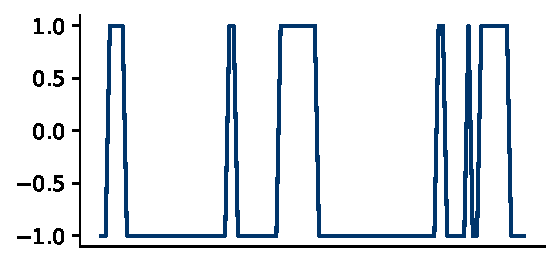
\includegraphics[height=\sampleheight]{figures/task/samples_long/ising.pdf} &
        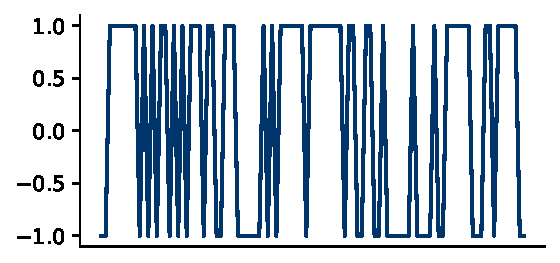
\includegraphics[height=\sampleheight]{figures/task/samples_short/ising.pdf} &
        \raisebox{38pt}{\rotatebox{90}{\tiny input dimension}} &
        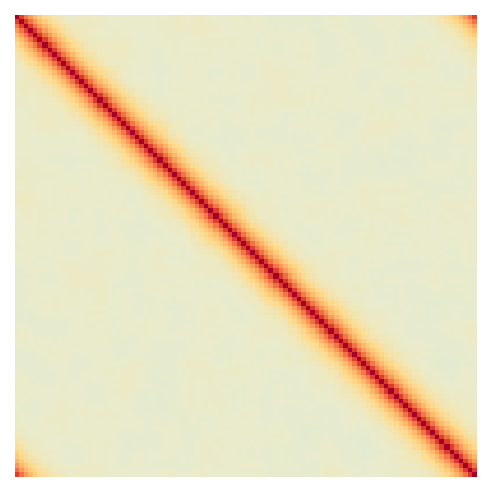
\includegraphics[height=\covheight]{figures/task/cov/ising.pdf} &
        \raisebox{40pt}{\rotatebox{90}{\tiny $p(X_i)$}} &
        \raisebox{-4pt}{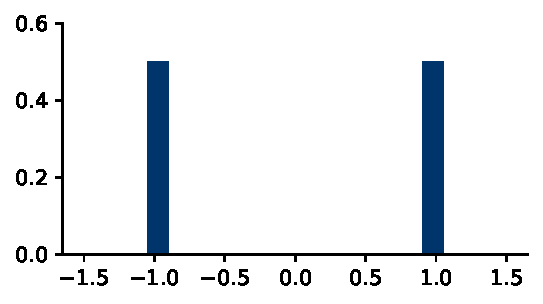
\includegraphics[height=\marginalheight]{figures/task/marginal/ising.pdf}} \\
        \noalign{\vskip -36pt}
        \raisebox{18pt}{\small$\texttt{NLGP}(0.01)$} &
        \raisebox{34pt}{\rotatebox{90}{\tiny input value}} &
        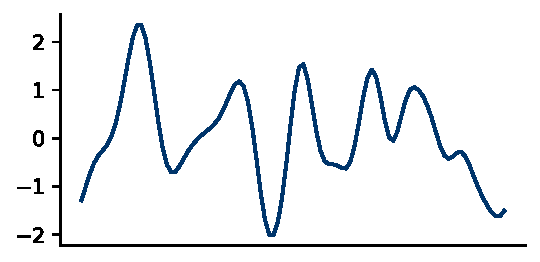
\includegraphics[height=\sampleheight]{figures/task/samples_long/gaussian.pdf} &
        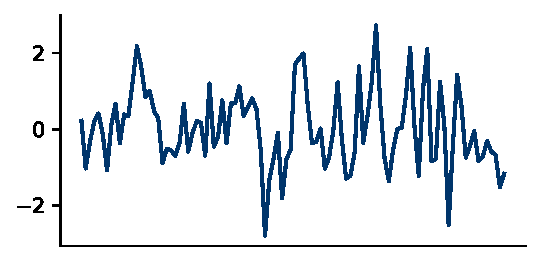
\includegraphics[height=\sampleheight]{figures/task/samples_short/gaussian.pdf} &
        \raisebox{38pt}{\rotatebox{90}{\tiny input dimension}} &
        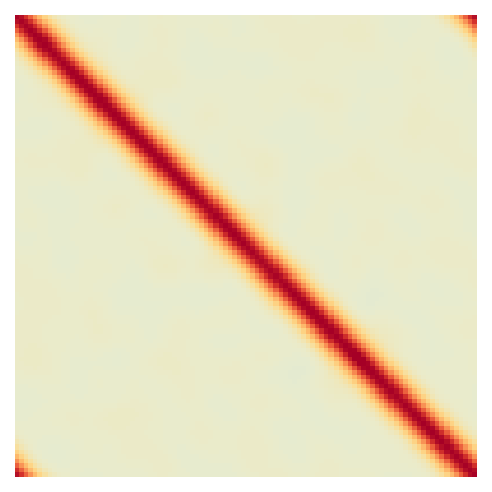
\includegraphics[height=\covheight]{figures/task/cov/gaussian.pdf} &
        \raisebox{40pt}{\rotatebox{90}{\tiny $p(X_i)$}} &
        \raisebox{-4pt}{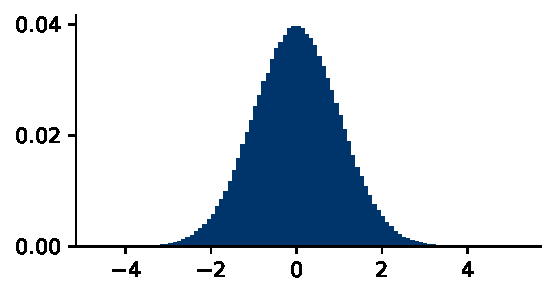
\includegraphics[height=\marginalheight]{figures/task/marginal/gaussian.pdf}} \\
        \noalign{\vskip -36pt}
        \raisebox{18pt}{\small $\texttt{Kur}(5)$} &
        \raisebox{34pt}{\rotatebox{90}{\tiny input value}} &
        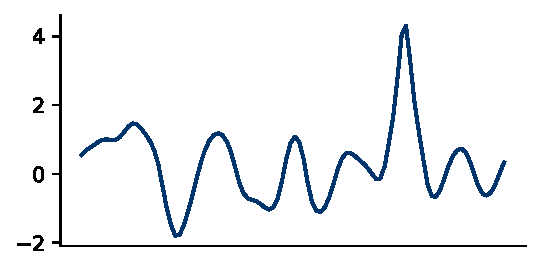
\includegraphics[height=\sampleheight]{figures/task/samples_long/alg5.pdf} &
        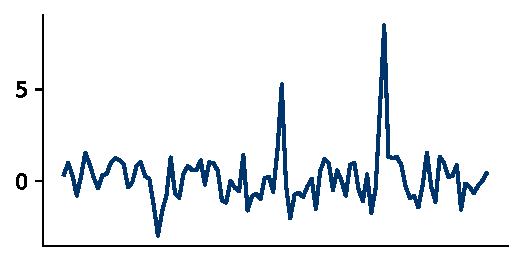
\includegraphics[height=\sampleheight]{figures/task/samples_short/alg5.pdf} &
        \raisebox{38pt}{\rotatebox{90}{\tiny input dimension}} &
        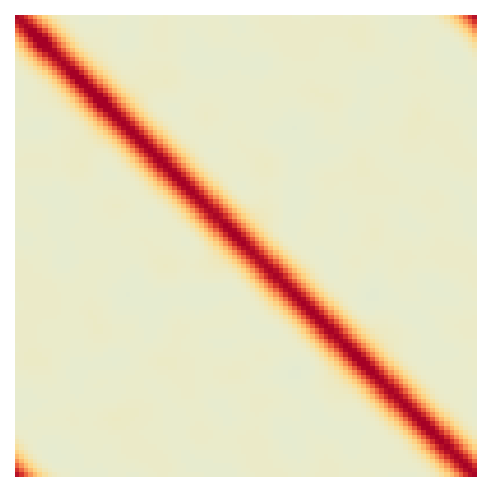
\includegraphics[height=\covheight]{figures/task/cov/alg5.pdf} &
        \raisebox{40pt}{\rotatebox{90}{\tiny $p(X_i)$}} &
        \raisebox{-4pt}{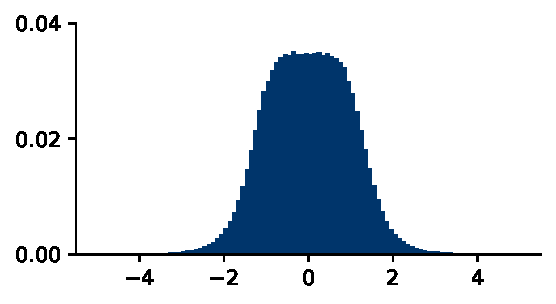
\includegraphics[height=\marginalheight]{figures/task/marginal/alg5.pdf}} \\
        \noalign{\vskip -37pt}
        &&
        \hspace{25pt}\tiny input dimension &
        \hspace{25pt}\tiny input dimension & &
        \hspace{3pt}\tiny input dimension & &
        \hspace{37pt}\tiny input value \\
  \end{tabular}
  \end{centering}
  }
  \caption{
    从左到右:
    长尺度和短尺度样本 $\mathbf{x}$,
    单一尺度的协方差 $\Sigma$,
    以及数据模型的边缘分布 $p(X_i)$,如 \cref{sec:task} 所述:
    Ising 模型(左、右样本分别为 $J=1.2, 0.3$),
    非线性高斯过程~\parencite[NLGP;~][]{ingrosso2022data},
    以及可控峰度模型 \texttt{Kur}
    (左、右样本分别为 $\xi=5, 1$)。
    \emph{
    每个模型生成的样本以零为中心,且其协方差可以被约束为相似,
    但具有不同的高阶统计量,从维度方向的边缘分布中可以看出这一点。
    }
}
  \label{fig:task}
  \vspace{-10pt}
\end{figure}


In \cref{fig:replications}, we validate Claim~\labelcref{thm:localization} first via the single-neuron model (\labelcref{item:single-neuron-model}) with 30 initial conditions trained across a range of excess kurtoses for the $\texttt{NLGP}(g)$ and $\texttt{Kur}(k)$ data models.
We use the inverse participation ratio (IPR), defined in \cref{app:IPR}.
This measure, also used by \textcite{ingrosso2022data}, is large when proportionally few weight dimensions ``participate'' (have large magnitude), and small when weight dimension magnitudes are more uniform.
We see that when $g$ and $k$ assume values that yield a negative excess kurtosis, IPR is close to its maximum of $1.0$, suggesting the weights are localized; if the excess kurtosis is positive, IPR is nearly zero, suggesting the weights are \emph{not} localized.
The IPR is extremely consistent across random initializations, suggesting that localization is determined by data statistics and not initialization.
The trend in IPR \vs excess kurtosis is very similar between the $\texttt{NLGP}(g)$ and $\texttt{Kur}(k)$ data models, demonstrating that excess kurtosis is a primary driver of localization and localization is largely independent from other properties of the data distribution.
\newcommand{\sampleheight}{42pt}
\newcommand{\covheight}{46pt}
\newcommand{\marginalheight}{50pt}
\setlength{\tabcolsep}{4pt}
\begin{figure}[t]
  \centering
  \hspace{-1.2em}
  \scalebox{0.9}{
  \begin{centering}
    \begin{tabular}{p{51pt}
      @{\hspace{10pt}}m{2pt}l
      @{\hspace{5pt}}l
      @{\hspace{10pt}}m{2pt}l
      @{\hspace{10pt}}m{2pt}l}
        \raisebox{18pt}{\small$\texttt{Ising}$} &
        \raisebox{34pt}{\rotatebox{90}{\tiny input value}} &
        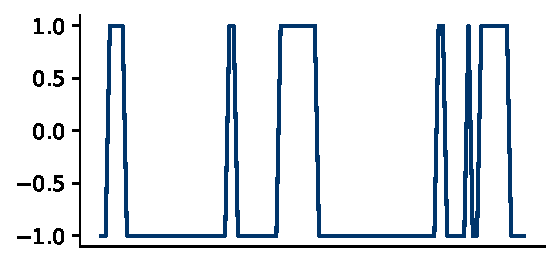
\includegraphics[height=\sampleheight]{figures/task/samples_long/ising.pdf} &
        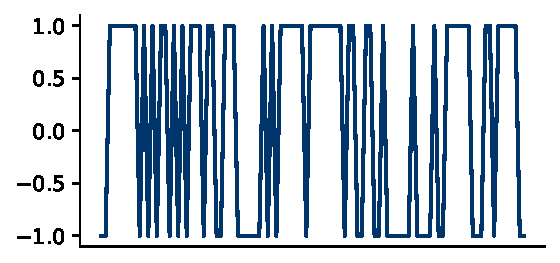
\includegraphics[height=\sampleheight]{figures/task/samples_short/ising.pdf} &
        \raisebox{38pt}{\rotatebox{90}{\tiny input dimension}} &
        \includegraphics[height=\covheight]{figures/task/cov/ising.pdf} &
        \raisebox{40pt}{\rotatebox{90}{\tiny $p(X_i)$}} &
        \raisebox{-4pt}{\includegraphics[height=\marginalheight]{figures/task/marginal/ising.pdf}} \\
        \noalign{\vskip -36pt}
        \raisebox{18pt}{\small$\texttt{NLGP}(0.01)$} &
        \raisebox{34pt}{\rotatebox{90}{\tiny input value}} &
        \includegraphics[height=\sampleheight]{figures/task/samples_long/gaussian.pdf} &
        \includegraphics[height=\sampleheight]{figures/task/samples_short/gaussian.pdf} &
        \raisebox{38pt}{\rotatebox{90}{\tiny input dimension}} &
        \includegraphics[height=\covheight]{figures/task/cov/gaussian.pdf} &
        \raisebox{40pt}{\rotatebox{90}{\tiny $p(X_i)$}} &
        \raisebox{-4pt}{\includegraphics[height=\marginalheight]{figures/task/marginal/gaussian.pdf}} \\
        \noalign{\vskip -36pt}
        \raisebox{18pt}{\small $\texttt{Kur}(5)$} &
        \raisebox{34pt}{\rotatebox{90}{\tiny input value}} &
        \includegraphics[height=\sampleheight]{figures/task/samples_long/alg5.pdf} &
        \includegraphics[height=\sampleheight]{figures/task/samples_short/alg5.pdf} &
        \raisebox{38pt}{\rotatebox{90}{\tiny input dimension}} &
        \includegraphics[height=\covheight]{figures/task/cov/alg5.pdf} &
        \raisebox{40pt}{\rotatebox{90}{\tiny $p(X_i)$}} &
        \raisebox{-4pt}{\includegraphics[height=\marginalheight]{figures/task/marginal/alg5.pdf}} \\
        \noalign{\vskip -37pt}
        &&
        \hspace{25pt}\tiny input dimension &
        \hspace{25pt}\tiny input dimension & &
        \hspace{3pt}\tiny input dimension & &
        \hspace{37pt}\tiny input value \\
  \end{tabular}
  \end{centering}
  }
  \caption{
    从左到右:
    长尺度和短尺度样本 $\mathbf{x}$,
    单一尺度的协方差 $\Sigma$,
    以及数据模型的边缘分布 $p(X_i)$,如 \cref{sec:task} 所述:
    Ising 模型(左、右样本分别为 $J=1.2, 0.3$),
    非线性高斯过程~\parencite[NLGP;~][]{ingrosso2022data},
    以及可控峰度模型 \texttt{Kur}
    (左、右样本分别为 $\xi=5, 1$)。
    \emph{
    每个模型生成的样本以零为中心,且其协方差可以被约束为相似,
    但具有不同的高阶统计量,从维度方向的边缘分布中可以看出这一点。
    }
}
  \label{fig:task}
  \vspace{-10pt}
\end{figure}


\Cref{fig:theory} further validates Claim~\labelcref{thm:localization} with specific examples.
We maintain constant initial conditions for our model and train on the \texttt{Ising}, $\texttt{NLGP}(g=0.01)$, and $\texttt{Kur}(k=5)$ data models.
The marginals of the \texttt{Ising} model have an excess kurtosis of $-2$, the smallest possible value for any distribution.
As a result, we see that the amplifier $\varphi$ for \texttt{Ising} (top left) is super-linear (the dark line exceeds the dashed light line for larger $a$), which drives localization via its role in \cref{eq:gradient_flow_early}.
Integrating \cref{eq:gradient_flow_early} with $\varphi$ expanded via a third-order Taylor approximation (red line) yields a similar localized receptive field to that from simulation (two right panels), validating this approximation.

For the remaining distributions (middle and bottom rows) that elicit oscillatory (sinusoidal) weights, 
Claim~\labelcref{thm:localization} is validated due to their positive excess kurtosis.
The dynamical steady state (far right) assumes a more negative value than in the simulation (to the left), 
a difference that is the result of deviations of our \emph{early-time} gradient flow in 
\cref{eq:gradient_flow_early}, but these deviations remain mild enough nevertheless to recover the qualitative structure of the learned receptive field.

\newcommand{\sampleheight}{42pt}
\newcommand{\covheight}{46pt}
\newcommand{\marginalheight}{50pt}
\setlength{\tabcolsep}{4pt}
\begin{figure}[t]
  \centering
  \hspace{-1.2em}
  \scalebox{0.9}{
  \begin{centering}
    \begin{tabular}{p{51pt}
      @{\hspace{10pt}}m{2pt}l
      @{\hspace{5pt}}l
      @{\hspace{10pt}}m{2pt}l
      @{\hspace{10pt}}m{2pt}l}
        \raisebox{18pt}{\small$\texttt{Ising}$} &
        \raisebox{34pt}{\rotatebox{90}{\tiny input value}} &
        \includegraphics[height=\sampleheight]{figures/task/samples_long/ising.pdf} &
        \includegraphics[height=\sampleheight]{figures/task/samples_short/ising.pdf} &
        \raisebox{38pt}{\rotatebox{90}{\tiny input dimension}} &
        \includegraphics[height=\covheight]{figures/task/cov/ising.pdf} &
        \raisebox{40pt}{\rotatebox{90}{\tiny $p(X_i)$}} &
        \raisebox{-4pt}{\includegraphics[height=\marginalheight]{figures/task/marginal/ising.pdf}} \\
        \noalign{\vskip -36pt}
        \raisebox{18pt}{\small$\texttt{NLGP}(0.01)$} &
        \raisebox{34pt}{\rotatebox{90}{\tiny input value}} &
        \includegraphics[height=\sampleheight]{figures/task/samples_long/gaussian.pdf} &
        \includegraphics[height=\sampleheight]{figures/task/samples_short/gaussian.pdf} &
        \raisebox{38pt}{\rotatebox{90}{\tiny input dimension}} &
        \includegraphics[height=\covheight]{figures/task/cov/gaussian.pdf} &
        \raisebox{40pt}{\rotatebox{90}{\tiny $p(X_i)$}} &
        \raisebox{-4pt}{\includegraphics[height=\marginalheight]{figures/task/marginal/gaussian.pdf}} \\
        \noalign{\vskip -36pt}
        \raisebox{18pt}{\small $\texttt{Kur}(5)$} &
        \raisebox{34pt}{\rotatebox{90}{\tiny input value}} &
        \includegraphics[height=\sampleheight]{figures/task/samples_long/alg5.pdf} &
        \includegraphics[height=\sampleheight]{figures/task/samples_short/alg5.pdf} &
        \raisebox{38pt}{\rotatebox{90}{\tiny input dimension}} &
        \includegraphics[height=\covheight]{figures/task/cov/alg5.pdf} &
        \raisebox{40pt}{\rotatebox{90}{\tiny $p(X_i)$}} &
        \raisebox{-4pt}{\includegraphics[height=\marginalheight]{figures/task/marginal/alg5.pdf}} \\
        \noalign{\vskip -37pt}
        &&
        \hspace{25pt}\tiny input dimension &
        \hspace{25pt}\tiny input dimension & &
        \hspace{3pt}\tiny input dimension & &
        \hspace{37pt}\tiny input value \\
  \end{tabular}
  \end{centering}
  }
  \caption{
    从左到右:
    长尺度和短尺度样本 $\mathbf{x}$,
    单一尺度的协方差 $\Sigma$,
    以及数据模型的边缘分布 $p(X_i)$,如 \cref{sec:task} 所述:
    Ising 模型(左、右样本分别为 $J=1.2, 0.3$),
    非线性高斯过程~\parencite[NLGP;~][]{ingrosso2022data},
    以及可控峰度模型 \texttt{Kur}
    (左、右样本分别为 $\xi=5, 1$)。
    \emph{
    每个模型生成的样本以零为中心,且其协方差可以被约束为相似,
    但具有不同的高阶统计量,从维度方向的边缘分布中可以看出这一点。
    }
}
  \label{fig:task}
  \vspace{-10pt}
\end{figure}

\subsection{Validating \cref{eq:gradient_flow_early} with localization position prediction}
\label{sec:peak-prediction}
The simulated and integrated receptive fields in \cref{fig:theory} demonstrate that our analytical model is able to meaningfully reproduce localization in receptive fields from neural network training.
For the Ising model, we see that the integration even has a peak in the exact same position as the simulation (at index $i=6$), suggesting precision in our approximation.
Indeed, we simulated the condition in \cref{fig:theory} for the Ising model under 28 different initial conditions (weight initializations), and found that in 26 of them (93\%), the peaks of the integrated and simulated receptive fields matched exactly.
In the two cases where the peaks differed, they did so substantially (see \cref{fig:time} for an example). 

\subsection{Validating Proposition \ref{thm:elliptical}: Elliptical distributions fail to localize}
\label{sec:elliptical-experiments}
Proposition \ref{thm:elliptical} claims that the single-neuron model (\labelcref{item:single-neuron-model})
trained on elliptical data will yield sinusoidal receptive fields, 
subject to a condition on the spectra of $\Sigma_0$ and $\Sigma_1$.
We verify this claim in \cref{fig:elliptical} with three distinct elliptical distributions.
The first, $t_{40}(\nu=3)$, gives preactivations $\langle \mathbf{w}, \mathbf{X} \rangle$ that have \emph{infinite} kurtosis, yet our theory predicts the final receptive field will be sinusoidal.
This is confirmed in \cref{fig:elliptical}, where the learned receptive field is indeed a sinusoid with period 1 and intercept at zero.

We also consider data sampled from the surface of an ellipse, which is done by fixing $R_y \equiv 1$ in \cref{def:elliptical}.
Here, we observe that the learned receptive field is a near-constant function at $-0.04$ (note that $\cos(2\pi \cdot 0 \cdot x) \equiv 1$ is a sinusoid, allowing nonzero intercepts and constant functions).
Finally, we consider an unconventional elliptical distribution where the density of $R$ is given by
$p_R(r) = (4e^{2r+4}) / (e^{2r}+e^{4})^{2} \cdot \mathbbm{1}(r \geq 2)$.
This particular density places most of its mass near $r = 2$ before rapidly falling off, imposing a minimum norm on $\mathbf{X}$ and pushing support near the surface of an ellipse.
This distribution, too, yields an oscillatory steady state, as shown in \cref{fig:elliptical} (right). 
We confirm our visual observations by fitting sinusoids to the final receptive fields and see the relative errors are quite low.

\subsection{Extensions to many-neuron model and ICA}
\label{sec:extensions}

All of our analysis thus far has concerned single-neuron models with ReLU activation and without hidden-to-output or bias terms, assumptions which were made to make our analysis tractable.
Here, we depart from that regime by considering the SCM and the full two-layer network (Model~\labelcref{item:many-neuron-model}).
In \cref{fig:extensions} (left) and (center), we train a SCM with 10 hidden units and sigmoid activation on the $\texttt{Kur}(10)$ and $\texttt{Kur}(4)$ datasets, which have excess kurtoses of $-0.93$ and $3.28$, respectively.
So, based on our single-neuron analysis, we \emph{do} and \emph{do not} expect to see localization for these distributions.
Indeed, this is precisely what we observe in \cref{fig:extensions}, where the receptive fields are sharply localized for the former distribution, while they look like low-frequency oscillations for the latter.

\newcommand{\sampleheight}{42pt}
\newcommand{\covheight}{46pt}
\newcommand{\marginalheight}{50pt}
\setlength{\tabcolsep}{4pt}
\begin{figure}[t]
  \centering
  \hspace{-1.2em}
  \scalebox{0.9}{
  \begin{centering}
    \begin{tabular}{p{51pt}
      @{\hspace{10pt}}m{2pt}l
      @{\hspace{5pt}}l
      @{\hspace{10pt}}m{2pt}l
      @{\hspace{10pt}}m{2pt}l}
        \raisebox{18pt}{\small$\texttt{Ising}$} &
        \raisebox{34pt}{\rotatebox{90}{\tiny input value}} &
        \includegraphics[height=\sampleheight]{figures/task/samples_long/ising.pdf} &
        \includegraphics[height=\sampleheight]{figures/task/samples_short/ising.pdf} &
        \raisebox{38pt}{\rotatebox{90}{\tiny input dimension}} &
        \includegraphics[height=\covheight]{figures/task/cov/ising.pdf} &
        \raisebox{40pt}{\rotatebox{90}{\tiny $p(X_i)$}} &
        \raisebox{-4pt}{\includegraphics[height=\marginalheight]{figures/task/marginal/ising.pdf}} \\
        \noalign{\vskip -36pt}
        \raisebox{18pt}{\small$\texttt{NLGP}(0.01)$} &
        \raisebox{34pt}{\rotatebox{90}{\tiny input value}} &
        \includegraphics[height=\sampleheight]{figures/task/samples_long/gaussian.pdf} &
        \includegraphics[height=\sampleheight]{figures/task/samples_short/gaussian.pdf} &
        \raisebox{38pt}{\rotatebox{90}{\tiny input dimension}} &
        \includegraphics[height=\covheight]{figures/task/cov/gaussian.pdf} &
        \raisebox{40pt}{\rotatebox{90}{\tiny $p(X_i)$}} &
        \raisebox{-4pt}{\includegraphics[height=\marginalheight]{figures/task/marginal/gaussian.pdf}} \\
        \noalign{\vskip -36pt}
        \raisebox{18pt}{\small $\texttt{Kur}(5)$} &
        \raisebox{34pt}{\rotatebox{90}{\tiny input value}} &
        \includegraphics[height=\sampleheight]{figures/task/samples_long/alg5.pdf} &
        \includegraphics[height=\sampleheight]{figures/task/samples_short/alg5.pdf} &
        \raisebox{38pt}{\rotatebox{90}{\tiny input dimension}} &
        \includegraphics[height=\covheight]{figures/task/cov/alg5.pdf} &
        \raisebox{40pt}{\rotatebox{90}{\tiny $p(X_i)$}} &
        \raisebox{-4pt}{\includegraphics[height=\marginalheight]{figures/task/marginal/alg5.pdf}} \\
        \noalign{\vskip -37pt}
        &&
        \hspace{25pt}\tiny input dimension &
        \hspace{25pt}\tiny input dimension & &
        \hspace{3pt}\tiny input dimension & &
        \hspace{37pt}\tiny input value \\
  \end{tabular}
  \end{centering}
  }
  \caption{
    从左到右:
    长尺度和短尺度样本 $\mathbf{x}$,
    单一尺度的协方差 $\Sigma$,
    以及数据模型的边缘分布 $p(X_i)$,如 \cref{sec:task} 所述:
    Ising 模型(左、右样本分别为 $J=1.2, 0.3$),
    非线性高斯过程~\parencite[NLGP;~][]{ingrosso2022data},
    以及可控峰度模型 \texttt{Kur}
    (左、右样本分别为 $\xi=5, 1$)。
    \emph{
    每个模型生成的样本以零为中心,且其协方差可以被约束为相似,
    但具有不同的高阶统计量,从维度方向的边缘分布中可以看出这一点。
    }
}
  \label{fig:task}
  \vspace{-10pt}
\end{figure}

In \cref{fig:multi-neuron}, we train many-neuron models with $N=40$ input units and $K=10$ hidden units, where all weights are learnable.
In general, adding flexibility in the second layer leads to more varied structure in the first layer.
We train on $\texttt{Kur}(4)$ (top), which has an excess kurtosis of $3.28$, and $\texttt{Kur}(30)$ (bottom), which has an excess kurtosis of $-1.17$.
The receptive fields from the former are not localized, as in the single-neuron model; however, they appear more like high-frequency oscillations than low-frequency sinusoids.
For $\texttt{Kur}(30)$, where we expect localization, we see that the first three receptive fields exhibit localization, but less so than for a single neuron.
Importantly, not all receptive fields are localized,
a result of a variable second-layer weight effectively changing the variance $\sigma^2$ in the third-derivative term in Lemma~\labelcref{lem:varphi}.

We further compare these predictions against ICA, another framework that has been used to model receptive fields in visual cortex.
We train on the $\texttt{Kur}(3)$ dataset, which has marginals with excess kurtosis $7.66$, fitting 10 components using the FastICA implementation from scikit-learn \parencite{hyvarinen2000independent,scikit-learn}.
We observe in \cref{fig:extensions} (right) that we learn localized receptive fields; this contrasts our neural network models, which require negative excess kurtosis.
This stems from ICA's objective to maximize non-Gaussianity, regardless of how specifically it is done.
The sign of the excess kurtosis is irrelevant, so long as it is nonzero.
This deviation between our analytical model and ICA is an interesting avenue for future study, perhaps by validation with natural images.

\section{Conclusions}
\label{sec:conclusions}

We derive effective learning dynamics for the minimal example of emergent localization in a neural receptive field given by \textcite{ingrosso2022data}. 
The analytical approach we take relies on the assumption that the \emph{conditional} preactivation is Gaussian, a refinement of previous work that assumes Gaussianity of the unconditioned preactivation as asserted by the \emph{Gaussian equivalence property} targeted by \textcite{ingrosso2022data}.
This approach may prove extensible beyond our specialized setting and may enable further analysis of how statistics of an input task drive emergent structure in neural network learning.

Emergence as an alternative mechanism to top-down constraints like sparsity
is in line with recent work that reformulates data-distributional properties as a driver for complex behavior~\parencite{chan2022data}. 
Via these analytical effective dynamics, we observe that specific data properties---the covariance structure 
and the marginals---shape localization in neural receptive fields.
Though we cannot capture dynamical interactions between neurons that may shape receptive fields in other settings with the single-neuron analytical model, our empirical validations with many neurons suggest that these interactions do not, in fact, play a significant role in shaping localization~\cite[\cf][]{harsh2020placecell}.

The data model we consider is a simplified abstraction of the task faced by early sensory systems, and, as a consequence, we do not yet capture certain features of receptive fields that are observed in early sensory systems.
In particular, we do not observe orientation nor phase selectivity, features of simple-cell receptive fields in early sensory cortices and in artificial neural networks that can be seen in a subset of receptive fields in \cref{fig:sim-real-gabors} (left and center, respectively).
To capture orientation selectivity, it may be fruitful to follow the approach of \textcite{karklin2011efficient}, who tie orientation selectivity in a population-based efficient-coding framework to the presence of noise.
Furthermore, on-center-off-surround-filtering input data, including the idealized data, gives receptive fields with subfields in our simulations, but is difficult to analyze.
Lastly, we do not yet look at the distribution of receptive field shapes and do not validate against other models of receptive field learning beyond a brief comparison with ICA~\parencite[\cf][]{saxe2011unsupervised}, but these are exciting avenues for future work.


\clearpage
\section*{Acknowledgements}
This work was supported by a Schmidt Science Polymath Award to A.S., and the Sainsbury Wellcome Centre Core Grant from Wellcome (219627/Z/19/Z) and the Gatsby Charitable Foundation (GAT3850). A.S. is a CIFAR Azrieli Global Scholar in the Learning in Machines \& Brains program.


\printbibliography

\clearpage
\appendix
\section{定义与符号}

\subsection{符号}
我们用 $[n]$ 来表示集合 $\{ i \in \N : 1 \leq i \leq n \}$。

\subsection{代数sigmoid函数}
\label{sec:algebraic-sigmoid}
对于 $k > 0$,广义代数sigmoid函数定义为
\begin{equation}
    \operatorname{alg}_k(x) \triangleq \frac{1}{2} \left( 1  + \frac{x}{(1+|x|^k)^{1/k}} \right)~.
\end{equation}
在后续的正文中,当 $k = 2$ 时,我们省略下标。
\subsection{反参与比(IPR)}  
\label{app:IPR}  
反参与比(IPR)定义为:  
$$ \operatorname{IPR}(\mathbf{w}) \triangleq \left(\sum_{i=1}^D w_i^4\right)/\left(\sum_{i=1}^D w_i^2\right)^2, $$  
其中,$w_i$ 表示权重 $\mathbf{w}$ 在第 $i$ 个维度上的幅值。
\section{超出主文范围的扩展}

\subsection{放大器 $\varphi$ 的解析性质}
\label{sec:varphi-analysis}

我们展示了在引理~\labelcref{lem:varphi} 中定义的放大函数 $\varphi$ 的几个性质。

\begin{lemma} \label{lem:varphi}
    局部放大器 $\varphi$ 在 \cref{eq:varphi} 中满足 $\varphi(-a) = -\varphi(a)$,对于所有 $a \in (-1,1)$ 都成立。  
    此外,其导数满足以下关系,其中 $\sigma^2$ 和 $\kappa$ 分别表示 $X_1$ 的方差和峰度:
    \vspace{-10pt}
    \begin{align*}
      \varphi'(0) &= \sqrt{\frac{2}{\pi}} \sigma^2~, &&\text { and }&&
      \varphi'''(0) = -\sqrt{\frac{2}{\pi}} (\kappa^4 \sigma^4 - 3 \sigma^2)~.
    \end{align*}
\end{lemma}
\vspace{-6pt}

为了更好地理解 $\mathbf{X}$ 的边际分布如何影响定位,我们使用引理~\labelcref{lem:varphi} 中的导数构造了关于 0 的 $\varphi$ 的三阶泰勒近似。
引理~\labelcref{lem:varphi} 中的导数表明,对于具有恒定方差的 $X_1$ 的每个分布,在 0 附近将表现为相同的线性函数。
只有当我们远离零时,第三阶项才变得重要,$\varphi$ 才表现为非线性。
在 $\sigma^2 = 1$ 的情况下(即 $X_1$ 的方差等于较大目标值 $y=1$),第三阶项表明当 $\kappa < 3$ 时,$\varphi$ 是超线性的,即过度峰度是正的,反之则为亚线性。

超线性的 $\varphi$ 会鼓励那些 $\Sigma_1 \mathbf{w}$ 较大的项比其他项以更快的速度增长,后者都通过 \cref{eq:gradient_flow_early} 中的第二项受到相同的 \emph{线性} 范数约束。
协方差矩阵 $\Sigma_1$ 作为循环矩阵,充当某些向量与 $\sigma_1^1$($\Sigma_1$ 的第一行)之间的卷积算子。
由于 $y=1$ 对应于具有较大长度尺度相关性的类别,$\sigma_1^1$ 会相对缓慢地衰减,像是一个加权的局部平均。
因此,$\Sigma_1 \mathbf{w}$ 是 $\mathbf{w}$ 中每个条目的加权局部平均。
因此,在某些邻域内,$\mathbf{w}$ 较大的条目将被鼓励比较小的条目增长得更快,这一效应会随着 \cref{eq:gradient_flow_early} 的积分而加剧。
因此,超线性促使定位。

正如我们将在引理~\ref{thm:elliptical} 中看到的,对于椭圆形数据的设置,如果 $\varphi$ 是线性的,$\mathbf{w}$ 会学习为正弦函数,因此不会定位。
在亚线性情况下,我们预期较大值会被抑制,而不是像超线性情况下那样被促进。
因此,首先近似地,过度峰度 $\kappa - 3$(对于 $\sigma^2 = 1$)的符号表明 $\mathbf{w}$ 是否定位。

然而,仅仅研究 $\varphi'''(0)$ 并不足以充分表征边际分布如何影响定位。
一个函数可能在小的 $a$ 下是亚线性的,而在较大的 $a$ 下是超线性的,这使得无法明确判断它是否会导致定位。
对于那些 $\kappa \approx 3$ 且没有表现出严格的超线性或亚线性的边际分布,这一条件已不再足够精确,无法确定是否会发生定位。
\subsection{方程 \cref{eq:gradient_flow_early} 的 PDE 极限}
\label{sec:pde-limit}

通过将 $N$ 取为较大并将 $w$ 视为与位置相关的连续函数,即 $w \equiv w(x, t)$,可以将 \cref{eq:gradient_flow_early} 视为偏微分方程(PDE)。  
求解其稳态等价于求解  
\begin{equation}
    \varphi\left( \frac{\sigma^1 \star w}{\sqrt{ \langle \sigma^1 \star w, w \rangle}} \right) - \frac{1}{2} (\sigma^0 + \sigma^1) \star w \equiv 0~,
\end{equation}  
其中 $w : [0,1] \to \R$ 是周期性的,$\sigma^y$ 是与矩阵 $\Sigma_y$ 极限情况对应的卷积。  
这个方程似乎没有非单位矩阵 $\Sigma_1$ 的显式解,因此,在这个 PDE 极限或对于有限 $N$ 时,可能无法精确求解 \cref{eq:gradient_flow_early} 的稳态。
\subsection{假设~\labelcref{item:mean-assumption,item:covariance-assumption} \vs 高斯等价性}

假设~\labelcref{item:mean-assumption,item:covariance-assumption} 等价于在训练初期将 $\langle \mathbf{w}, \mathbf{X} \rangle \mid X_i$ 近似为高斯分布。
类似的思想已被用于推导神经网络的梯度流动力学,包括在建立高斯等价性性质的研究中,如 \cite{goldt2020modelling,gerace2020generalisation,goldt2022gaussian}。
然而,这些工作建模的是无条件的预激活项 $\langle \mathbf{w}, \mathbf{X} \rangle$ 为高斯分布,而不是首先对 $X_i$ 进行条件化。
其产生的原因在于,这些先前的工作是在对损失函数进行梯度流动力学求导 \emph{之前} 就提出了高斯近似。
但在该阶段进行近似会忽略一个乘性因子 $\mathbf{X}$,这是由于链式法则作用于 $\langle \mathbf{w}, \mathbf{X} \rangle$ 所导致的。
从抽象角度来看,这种方法假设 $\LL_\text{exact} \to \LL_\text{Gauss}$ 推出 $\nabla_\mathbf{w} \LL_\text{exact} \to \nabla_\mathbf{w} \LL_\text{Gauss}$,但一般来说这一推理并不成立,尤其在此处,这一假设未能体现学习过程与高阶输入统计量之间的相互作用。
这也是 \cite{ingrosso2022data} 中高斯等价性失败的一个原因。
相比之下,在推导引理~\labelcref{lem:gradient_flow} 时,我们可以通过假设 $\langle \mathbf{w}, \mathbf{X} \rangle \mid X_i$ 而不是 $\langle \mathbf{w}, \mathbf{X} \rangle$ 是高斯分布,从而考虑额外的 $\mathbf{X}$ 项。
这种条件化的方法,加之数据的平移不变性(性质~\labelcref{item:translation-invariance}),也进一步激发了将边缘分布 $X_i$ 作为研究对象的动机,以获得适用于非高斯输入训练的神经网络的梯度流。
\section{理论结果的证明}
\label{app:proofs}

\subsection{均方误差(MSE)损失的梯度流}
损失函数由以下给出:
\begin{align}
    \LL
    &= \E_{\mathbf{X},Y}\left[ (Y - \operatorname{ReLU}(\langle \mathbf{w}, \mathbf{X} \rangle) )^2 \right] \notag \\
    &= \E_{\mathbf{X},Y}\left[ Y^2 \right] - 2 \underbrace{ \E_{\mathbf{X},Y}\left[ Y \operatorname{ReLU}(\langle \mathbf{w}, \mathbf{X} \rangle) \right] }_{\triangleq (I)} + \underbrace{ \E_{\mathbf{X},Y}\left[ \operatorname{ReLU}^2(\langle \mathbf{w}, \mathbf{X} \rangle) \right] }_{\triangleq (II)}. \label{eq:loss_2relu_neuron}
\end{align}
符号对称性假设(\labelcref{item:sign-symmetry})表明
$\langle \mathbf{w}, \mathbf{X} \rangle$ 也具有符号对称性。
首先,这意味着 $\PR( \langle \mathbf{w}, \mathbf{X} \rangle > 0 ) = \frac{1}{2}$,所以:
\begin{align*}
    (II)
    &= \frac{1}{2} \E_{\mathbf{X},Y \mid \langle \mathbf{w}, \mathbf{X} \rangle \geq 0}\left[ \operatorname{ReLU}^2(\langle \mathbf{w}, \mathbf{X} \rangle) \right]
    = \frac{1}{2} \E_{\mathbf{X},Y \mid \langle \mathbf{w}, \mathbf{X} \rangle \geq 0}\left[ (\langle \mathbf{w}, \mathbf{X} \rangle)^2 \right].
\end{align*}
其次,$\langle \mathbf{w}, \mathbf{X} \rangle$ 的符号对称性
意味着我们可以去掉条件 $\langle \mathbf{w}, \mathbf{X} \rangle \geq 0$,因为 $\langle \mathbf{w}, \mathbf{X} \rangle \overset{d}{=} -\langle \mathbf{w}, \mathbf{X} \rangle$。
因此,
\begin{align*}
    (II)
    &= \frac{1}{2} \E_{\mathbf{X},Y}\left[ (\langle \mathbf{w}, \mathbf{X} \rangle)^2 \right] \\
    &= \frac{1}{2} \mathbf{w}^\top \E_{\mathbf{X},Y} \left[ \mathbf{X} \mathbf{X}^\top \right] \mathbf{w} \\
    &= \frac{1}{2} \mathbf{w}^\top \left( \frac{1}{K} \sum_{y=0}^{K-1} \Sigma_y \right) \mathbf{w}  \\
    &= \frac{1}{2K} \sum_{y=0}^{K-1} \mathbf{w}^\top \Sigma_y \mathbf{w}~,
\end{align*}
其中 $K$ 是离散的 $y$ 的值(类别)数。
最后,我们对 $\mathbf{w}$ 对损失函数 $\LL$ 求导:
\begin{align*}
  \nabla_\mathbf{w} \LL &= 2 \E_{\mathbf{X},Y}\left[ Y \mathbbm{1}( \langle \mathbf{w}, \mathbf{X} \rangle \geq 0) \mathbf{X} \right] + \frac{1}{K} \sum_{y=0}^{K-1} \Sigma_y \mathbf{w}~.
\end{align*}
梯度流~\cite{elkabetz2024continuous}由 $\frac{\mathrm{d}\mathbf{w}}{\mathrm{d}t} = -\tau \nabla_\mathbf{w} \LL$ 给出,其中 $\tau$ 是学习率。
因此,
\begin{equation}
  \frac{1}{\tau} \frac{\mathrm{d}\mathbf{w}}{\mathrm{d}t}
    = 2 \E_{\mathbf{X},Y}\left[ Y \mathbbm{1}( \langle \mathbf{w}, \mathbf{X} \rangle \geq 0) \mathbf{X} \right] - \frac{1}{K} \sum_{y=1}^{K} \Sigma_y \mathbf{w}~. \label{eq:gradient_flow_two}
\end{equation}
\subsection{引理 \ref{lem:gradient_flow} 的证明} \label{subsec:pf_of_gradient_flow}
在方程 \eqref{eq:gradient_flow_two} 中设定 $K = 2$,我们得到
\begin{align*}
  \frac{1}{\tau} \frac{\mathrm{d}\mathbf{w}}{\mathrm{d}t}
  &= \E_{\mathbf{X} \mid Y=1}[ \mathbbm{1}( \langle \mathbf{w}, \mathbf{X} \rangle \geq 0 ) \mathbf{X} ] - \frac{1}{2} \left( \Sigma_0 + \Sigma_1 \right) \mathbf{w}~.
\end{align*}
我们希望显式地表示第一项。
注意,第一项是 $\R^N$ 中的一个向量。
我们通过使用全期望法则,分别考虑每一项,写出第 $i$ 项为:
\begin{align*}
    \E_{\mathbf{X} \mid Y=1}[ \mathbbm{1}( \langle \mathbf{w}, \mathbf{X} \rangle \geq 0 ) X_i ]
    &= \E_{ X_i \mid Y=1 } \left[ X_i \PR_{\mathbf{X} \mid X_i=x_i, Y = 1} \left[  \langle \mathbf{w}, \mathbf{X} \rangle \geq 0 \right] \right]~.
\end{align*}

根据假设~\labelcref{item:lindeberg-condition},$\{ w_i X_i \mid 1 \leq i \leq N \}$ 满足 Lindeberg 条件,当 $N \to \infty$ 时。
这也被称为 \emph{一致可积性} 要求。
在正式阐述之前,首先引入两个变量:$S_N \triangleq \sum_{j=1}^{N} w_j (X_j - \mu_{j\mid x_i})$,部分和,以及它们的方差,$\sigma_N^2 \triangleq \E[ S_N^2 ]$,其中 $\mu_{j \mid x_i} \triangleq \E[X_j \mid X_i = x_i]$ 是在给定第 $i$ 项值为 $x_i$ 时,第 $j$ 项的条件均值。
然后,Lindeberg 条件被正式表述为
\begin{equation*}
  \sup_N \E_{S_N \mid X_i = x_i} \left[ \left| \tfrac{S_N^2}{\sigma_N^2} \right| \mathbbm{1} \left( \left| \tfrac{S_N^2}{\sigma_N^2} \right| > x \right) \right] \to 0 \quad \text{as} \quad x\to\infty~.
\end{equation*}
该条件实际上表明,部分和中的任何项 $w_i X_i$ 都不会占主导地位。
在该条件下,结合弱依赖性(性质~\labelcref{item:weak-dependence}),我们根据 \cite[定理 1.19, 10.2]{bradley2007introduction} 得出 $S_N / \sigma_N \overset{d}{\to} \NN(0,1)$。
注意到
\begin{equation*}
    S_N = \langle \mathbf{w}, \mathbf{X} \rangle - \langle \mathbf{w}, \mathbf{\mu}_{\mid x_i} \rangle \qquad  \text{and} \qquad \sigma_N = \sqrt{\mathbf{w}^\top \Sigma_{\mid x_i}^{1} \mathbf{w}}~,
\end{equation*}
其中,$\mathbf{w}, \mathbf{X}$ 是 $N$ 维向量,$\mathbf{\mu}_{\mid x_i} = \E[\mathbf{X} \mid X_i = x_i]$ 是条件均值的向量,而 $\Sigma_{\mid x_i}^{1} \triangleq \text{Cov}[\mathbf{X} \mid X_i = x_i, Y = 1] = \Sigma_1 - \sigma_i^1 \sigma_i^{1\top}$。
由于 $\sigma_N$ 和 $\mathbf{\mu}_{\mid x_i}$ 是常数,我们可以写作
\begin{align*}
    \PR_{\mathbf{X} \mid X_i = x_i, Y = 1} \left[  \langle \mathbf{w}, \mathbf{X} \rangle \geq 0 \right]
    &= \PR_{\mathbf{X} \mid X_i, Y = 1} \left[ \frac{ \langle \mathbf{w}, \mathbf{X} \rangle - \langle \mathbf{w}, \mathbf{\mu}_{j \mid x_i} \rangle }{ \sigma_N } \geq -\frac{\langle \mathbf{w}, \mathbf{\mu}_{j \mid x_i} \rangle }{ \sigma_N } \right] \\
    &= \PR_{Z \sim \NN(0,1)} \left[ Z \geq -\frac{\langle \mathbf{w}, \mathbf{\mu}_{j \mid x_i} \rangle }{ \sigma_N } \right] + o_N(1) \\
    &= 1 - \frac{1}{2} \left[ 1 + \operatorname{erf}\left( -\frac{\langle \mathbf{w}, \mathbf{\mu}_{j \mid x_i} \rangle }{ \sqrt{2} \sigma_N } \right) \right] + o_N(1) \\
    &= \frac{1}{2} + \frac{1}{2} \operatorname{erf}\left(\frac{\langle \mathbf{w}, \mathbf{\mu}_{j \mid x_i} \rangle }{ \sqrt{2} \sigma_N } \right) + o_N(1)~,
\end{align*}
其中第二步,得到 $o_N(1)$,是由分布收敛的定义得出的。
在假设 \labelcref{item:mean-assumption,item:covariance-assumption} 下,我们可以将其表示为
\begin{align*}
    \PR_{\mathbf{X} \mid X_i = x_i, Y = 1} \left[  \langle \mathbf{w}, \mathbf{X} \rangle \geq 0 \right]
    &= \frac{1}{2} + \frac{1}{2} \operatorname{erf}\left( \frac{\langle \mathbf{w}, x_i \sigma_i^y \rangle }{ \sqrt{2} \sqrt{ \mathbf{w}^\top \Sigma_1 \mathbf{w} - (\langle \mathbf{w}, \sigma_i^y \rangle)^2 } } \right) + o_N(1)~.
\end{align*}
因此,
\begin{align*}
    &\E_{\mathbf{X} \mid Y=1}[ \mathbbm{1}( \langle \mathbf{w}, \mathbf{X} \rangle \geq 0 ) X_i ] \\
    &= \E_{ X_i \mid Y=1 } \left[ X_i \left( \frac{1}{2} + \frac{1}{2} \operatorname{erf}\left( \frac{X_i}{\sqrt{2}} \cdot \frac{\langle \mathbf{w}, \sigma_i^y \rangle }{ \sqrt{ \mathbf{w}^\top \Sigma_1 \mathbf{w} - (\langle \mathbf{w}, \sigma_i^y \rangle)^2 } } \right) + o_N(1) \right) \right] \\
    &= \frac{1}{2} \E_{ X_i \mid Y=1 } \left[ X_i \operatorname{erf}\left( \frac{X_i}{\sqrt{2}} \cdot \frac{\langle \mathbf{w}, \sigma_i^y \rangle / \sqrt{\mathbf{w}^\top \Sigma_1 \mathbf{w}} }{ \sqrt{ 1 - (\langle \mathbf{w}, \sigma_i^y \rangle / \sqrt{\mathbf{w}^\top \Sigma_1 \mathbf{w}})^2 } } \right) \right] + \E_{X_i}[|X_i|] o_N(1) \\
    &= \frac{1}{2} \E_{ X_i \mid Y=1 } \left[ X_i \operatorname{erf}\left( \frac{X_i}{\sqrt{2}} \cdot \operatorname{alg}^{-1} \left( \frac{ \langle \mathbf{w}, \sigma_i^y \rangle }{ \sqrt{\mathbf{w}^\top \Sigma_1 \mathbf{w}} } \right) \right) \right] + \E_{X_i}[|X_i|] o_N(1)~.
\end{align*}
定义 $\varphi_i(a) \triangleq \E_{X_i \mid Y=1}[ X_i \operatorname{erf}(X_i \operatorname{alg}^{-1}(a) / \sqrt{2}) ]$,我们可以写作
\begin{align*}
    \E_{\mathbf{X} \mid Y=1}[ \mathbbm{1}( \langle \mathbf{w}, \mathbf{X} \rangle \geq 0 ) X_i ]
    &= \frac{1}{2} \varphi_i \left( \frac{ \langle \mathbf{w}, \sigma_i^y \rangle }{ \sqrt{\mathbf{w}^\top \Sigma_1 \mathbf{w}} } \right) + \E_{X_i}[|X_i|] o_N(1)~.
\end{align*}
注意,由于 Cauchy-Schwarz 不等式,$\E_{X_i}[|X_i|] \leq \sqrt{ \E_{X_i}[X_i^2] } = \sigma$。
所以,$\E_{X_i}[|X_i|] o_N(1) = o_N(1)$。
此外,由于平移不变性,所有的 $X_i$ 具有相同的边际分布,因此 $\varphi_i \equiv \varphi_1 \triangleq \varphi$。
因此,
\begin{align*}
    \E_{\mathbf{X} \mid Y=1}[ \mathbbm{1}( \langle \mathbf{w}, \mathbf{X} \rangle \geq 0 ) X_i ]
    &= \frac{1}{2} \varphi \left( \frac{ \langle \mathbf{w}, \sigma_i^y \rangle }{ \sqrt{\mathbf{w}^\top \Sigma_1 \mathbf{w}} } \right) + o_N(1)~.
\end{align*}
这个形式对于所有项 $i$ 都成立。
将它们连接起来,我们得到
\begin{align*}
    \E_{\mathbf{X} \mid Y=1}[ \mathbbm{1}( \langle \mathbf{w}, \mathbf{X} \rangle \geq 0 ) \mathbf{X} ]
    &= \frac{1}{2} \varphi \left( \frac{ \Sigma_1 \mathbf{w} }{ \sqrt{\mathbf{w}^\top \Sigma_1 \mathbf{w}} } \right) + o_N(1)~,
\end{align*}
从而得到所需的结果。
\qed
\subsection{引理 \ref{lem:varphi} 的证明} \label{subsec:pf_of_varphi}
性质 1 来源于 $\operatorname{alg}$ 和 $\operatorname{erf}$ 是奇函数这一事实。这意味着性质 4 得以成立,因为奇函数的偶次 Taylor 系数必须为零。

性质 2 和 3 来源于对 \cref{eq:varphi} 求导。第一导数为
\begin{align*}
    \varphi'(a) &= \frac{\sqrt{2}}{{\sqrt{{\pi}}}(1-a^2)^\frac{3}{2}} \E_{X_1}\left[ X_1^2\mathrm{e}^{-\frac{X_1^2a^2}{2(1-a^2)}} \right].
\end{align*}
设置 $a = 0$,我们得到
\begin{align*}
    \varphi'(0)
    &= \sqrt{\frac{2}{\pi}} \E\left[ X_1^2 \right]
    = \sqrt{\frac{2}{\pi}} \sigma^2.
\end{align*}
第三导数为
\begin{align*}
    \varphi'''(a) &= \frac{\sqrt{2}}{\sqrt{{\pi}}(1-a^2)^\frac{7}{2}(a^2-1)^2} \E_{X_1} \left[
    X_1^2(12a^6+(9X_1^2-21)a^4+(X_1^4-8X_1^2+6)a^2-X_1^2+3)\mathrm{e}^{-\frac{X_1^2a^2}{2(1-a^2)}}
    \right].
\end{align*}
再次设置 $a = 0$ 得到
\begin{align*}
    \varphi'''(0) &= \sqrt{\frac{2}{\pi}} \E_{X_1} \left[ X_1^2(-X_1^2+3) \right]
    = \sqrt{\frac{2}{\pi}} \left( 3 \E_{X_1}[X_1^2] - \E_{X_1}[X_1^4] \right)
    = -\sqrt{\frac{2}{\pi}} (\kappa^4 \sigma^4 - 3 \sigma^2)~.
\end{align*}
\qed
\subsection{命题~\ref{thm:elliptical}的证明}
$X \sim \EE_N(\mu, \Sigma, \phi)$的pdf为
\begin{align*}
    p_X(x) &= \frac{1}{\sqrt{\det(\Sigma)}} g( (x-\mu)^\top \Sigma^{-1} (x-\mu) )~,
\end{align*}
对于某个函数$g : \R_{\geq 0} \to \R_{\geq 0}$ \cite{frahm2004generalized}。
椭圆分布的一个关键性质是,如果$X \sim \EE_N(\mu, \Sigma, \phi)$,则其仿射变换也是椭圆分布:$\langle \mathbf{w}, \mathbf{X} \rangle \sim \EE_1(\langle \mathbf{w}, \mu \rangle, \mathbf{w}^\top \Sigma \mathbf{w}, \phi)$,对于任何$\mathbf{w} \in \R^N$。
因此,
\begin{align*}
  p_{\langle \mathbf{w}, \mathbf{X} \rangle}(s) &= \frac{1}{\sqrt{\mathbf{w}^\top \Sigma \mathbf{w}}} \tilde{g}\left( \frac{(s-\langle \mathbf{w}, \mu \rangle)^2}{\mathbf{w}^\top \Sigma \mathbf{w}} \right),
\end{align*}
对于另一个函数$\tilde{g} : \R_{\geq 0} \to \R_{\geq 0}$。

根据我们的符号对称性假设,我们有$\mu = 0$。
为了简便起见,我们定义$\sigma^2 \triangleq \mathbf{w}^\top \Sigma \mathbf{w}$和$S \triangleq \langle \mathbf{w}, \mathbf{X} \rangle$。
我们首先计算\cref{eq:loss_2relu_neuron}中的(I)。
回忆一下,我们有$y = 0,1$(即$K = 2$)。
所以,
\begin{align*}
    2 \times (I)
    &= \E_{S \mid Y=1}[ \operatorname{ReLU}( S ) ]
    = \int_0^{\infty} \frac{1}{\sigma} \tilde{g}\left( \frac{s^2}{\sigma^2} \right) s \ \mathrm{d}s.
\end{align*}
此时,我们对$u = s^2 / \sigma^2$进行$u$-代换,因此$\mathrm{d}u = 2 s \ \mathrm{d}s / \sigma^2 \iff \sigma \mathrm{d}u / 2 = s\ \mathrm{d}s / \sigma$。
这给出
\begin{align*}
    2 \times (I)
    &= \frac{\sigma}{2} \underbrace{\int_0^{\infty} \tilde{g}(u)\ \mathrm{d}u}_{\triangleq C}
    = \frac{C}{2} \sqrt{\mathbf{w}^\top \Sigma_1 \mathbf{w}}.
\end{align*}
回忆一下,我们假设MSE损失$\LL$是有限的。
\cref{eq:loss_2relu_neuron}中的第一项显然对于$y = 0,1$是有限的。
项$(II)$也容易看出是有限的,因为它等于$\mathbf{w}^\top (\Sigma_0 + \Sigma_1) \mathbf{w} / 4$。
因此,$\LL$是有限的意味着\cref{eq:loss_2relu_neuron}中的(I)是有限的,这意味着$C < \infty$。
我们从上面的\cref{eq:loss_2relu_neuron}中计算了(II)为
\begin{align*}
  \frac{1}{4} \mathbf{w}^\top \left( \Sigma_0 + \Sigma_1 \right) \mathbf{w}
\end{align*}
对于$K = 2$。
将(I)和(II)代入并对$\mathbf{w}$求导,我们得到
\begin{equation}
  \frac{1}{\tau} \frac{\mathrm{d}\mathbf{w}}{\mathrm{d}t} = \frac{\Sigma_1 \mathbf{w}}{\sqrt{\mathbf{w}^\top \Sigma_1 \mathbf{w}}} - \frac{1}{2} \left( \Sigma_0 + \Sigma_1 \right) \mathbf{w}~. \label{eq:elliptical_gradient_flow}
\end{equation}
因此,\cref{eq:elliptical_gradient_flow}的稳态满足
\begin{align*}
  C \frac{\Sigma_1 \mathbf{w}}{\sqrt{\mathbf{w}^\top \Sigma_1 \mathbf{w}}}
  &= \frac{1}{2} \left( \Sigma_0 + \Sigma_1 \right) \mathbf{w}~.
\end{align*}
回忆一下,平移不变性意味着$\Sigma_0$和$\Sigma_1$是循环矩阵,并且由于它们是协方差矩阵,因此它们是对称的。
然后,它们在由离散傅里叶变换中前$n/2$个傅里叶分量的实部和虚部给出的基中对角化,我们用$n \times n$实矩阵$\FF$表示。
注意$\FF$是正交的。
定义$\mathbf{v} = \FF^\top \mathbf{w}$和$\Lambda_y = \FF^\top \Sigma_y \FF$,其中$y = 0,1$。
因此,稳态满足
\begin{align*}
  C \frac{\Lambda_1 \mathbf{v}}{\sqrt{\mathbf{v}^\top \Lambda_1 \mathbf{v}}} &= \frac{1}{2} \left( \Lambda_0 + \Lambda_1 \right) \mathbf{v}~.
\end{align*}
当且仅当对于所有$i \in [n]$,
\begin{align*}
  C (\Lambda_1)_{ii} (\mathbf{v}^\top \Lambda_1 \mathbf{v})^{-\frac{1}{2}} v_i &= \frac{1}{2} ( (\Lambda_0)_{ii} + (\Lambda_1)_{ii} ) v_i~.
\end{align*}
因此,如果$v_i \neq 0$,我们必须有
\begin{align*}
  \frac{(\Lambda_0)_{ii}}{(\Lambda_1)_{ii}} &= 2 C (\mathbf{v}^\top \Lambda_1 \mathbf{v})^{-\frac{1}{2}} - 1~.
\end{align*}
也就是说,$\Sigma_0$和$\Sigma_1$的第$i$个特征值的比率必须对于所有$v_i \neq 0$的$i$保持不变。
由于我们使用离散傅里叶变换定义了$\FF$,这些矩阵的特征值总是成对出现。
通常,我们观察到每对特征值都有唯一的值。
因此,由于$C$是有限的,上述条件至多可以在两个不同的$i$值下成立。
因此,除最多两个$i \in [n]$外,$v_i = 0$,这意味着稳态$w$的形式为$a \cos(2\pi k x) + b \sin(2 \pi k x)$,即它是振荡的。
因此,它是\emph{非}局部化的。
\qed

\section{附加实验}

\subsection{可视化假设~\labelcref{item:lindeberg-condition} 的分解}

\cref{fig:time} 展示了我们的分析模型在训练过程中足够长的时间内有效,能够捕捉到单个 ReLU 神经元中的定位现象(\labelcref{item:single-neuron-model})。
在前面三列中,我们可视化了来自我们经验模型和分析模型的权重的 IPR,以及这两个权重之间的 $\ell_2$ 差异。
在前四行中,我们可视化了这些指标,分别对应模型的四个随机初始化,每个初始化在 $\texttt{NLGP}(g=100)$ 上训练,且 $\xi_0 = 0.3$ 和 $\xi_1 = 0.7$,根据 \cref{thm:localization},我们期望看到定位现象。
我们看到,在 IPR 增加后不久,误差迅速增加,表明局部感受野的形成。
最后三列确认了这一点,它们展示了在经验权重和分析权重之间的发散发生前、中、后的快照。
我们观察到,权重在 \emph{之前} 几乎完全相同,在 \emph{期间} 最局部化的点仅有微小差异,而在 \emph{之后} 都是局部化的,但可能具有不同的幅度和位置。
在 \emph{期间} 出现的差异是由于假设~\labelcref{item:lindeberg-condition} 的失效,这个假设在构建我们的分析模型时使用,当 $\mathbf{w}$ 的范数被少数几项主导时(即局部化时)会被违背。
虽然 \cite{ingrosso2022data} 也观察到他们的分析模型在局部化出现时发生崩溃,但我们的方法关键地在足够长的时间内有效,从而能够表征局部化的出现。

我们将对各个子图进行更详细的讨论。
在 \cref{fig:time} 的所有行中,除了第三行,分析预测几乎完全准确;在第三行中,我们预测了定位现象,但位置错误。
再次聚焦在第一行,我们看到在 $t=20$ 时,权重尚未局部化(从 IPR 左侧、第一列和视觉上来看),分析权重和经验权重几乎完全一致,这一点可以通过左侧、中心上方的小距离确认。
在 $t=30$ 时,围绕 $i=21$ 的局部峰值开始出现,这违背了假设 \labelcref{item:lindeberg-condition},并削弱了分析精度。
分析模型低估了主峰 $i=21$ 的主导程度,同时高估了 $i=30$、$37$ 和 $90$ 处竞争峰的大小。
尽管如此,在 $t=50$ 时,我们看到分析模型的预测仍然与经验模型相匹配。

在 \cref{fig:time} 的最后一行,我们使用与第一行相同的初始化和设置,只不过我们改为在 $\texttt{NLGP}(g=0.01)$ 数据上进行训练。
根据 \cref{thm:localization},我们\emph{不}期望看到定位现象。
IPR 的演化确认了这一点,因为它保持在较低的幅度。
我们还观察到,由于定位现象从未出现,假设~\labelcref{item:lindeberg-condition} 从未被违背,因此我们的分析模型几乎完全符合经验模型。

\newcommand{\sampleheight}{42pt}
\newcommand{\covheight}{46pt}
\newcommand{\marginalheight}{50pt}
\setlength{\tabcolsep}{4pt}
\begin{figure}[t]
  \centering
  \hspace{-1.2em}
  \scalebox{0.9}{
  \begin{centering}
    \begin{tabular}{p{51pt}
      @{\hspace{10pt}}m{2pt}l
      @{\hspace{5pt}}l
      @{\hspace{10pt}}m{2pt}l
      @{\hspace{10pt}}m{2pt}l}
        \raisebox{18pt}{\small$\texttt{Ising}$} &
        \raisebox{34pt}{\rotatebox{90}{\tiny input value}} &
        \includegraphics[height=\sampleheight]{figures/task/samples_long/ising.pdf} &
        \includegraphics[height=\sampleheight]{figures/task/samples_short/ising.pdf} &
        \raisebox{38pt}{\rotatebox{90}{\tiny input dimension}} &
        \includegraphics[height=\covheight]{figures/task/cov/ising.pdf} &
        \raisebox{40pt}{\rotatebox{90}{\tiny $p(X_i)$}} &
        \raisebox{-4pt}{\includegraphics[height=\marginalheight]{figures/task/marginal/ising.pdf}} \\
        \noalign{\vskip -36pt}
        \raisebox{18pt}{\small$\texttt{NLGP}(0.01)$} &
        \raisebox{34pt}{\rotatebox{90}{\tiny input value}} &
        \includegraphics[height=\sampleheight]{figures/task/samples_long/gaussian.pdf} &
        \includegraphics[height=\sampleheight]{figures/task/samples_short/gaussian.pdf} &
        \raisebox{38pt}{\rotatebox{90}{\tiny input dimension}} &
        \includegraphics[height=\covheight]{figures/task/cov/gaussian.pdf} &
        \raisebox{40pt}{\rotatebox{90}{\tiny $p(X_i)$}} &
        \raisebox{-4pt}{\includegraphics[height=\marginalheight]{figures/task/marginal/gaussian.pdf}} \\
        \noalign{\vskip -36pt}
        \raisebox{18pt}{\small $\texttt{Kur}(5)$} &
        \raisebox{34pt}{\rotatebox{90}{\tiny input value}} &
        \includegraphics[height=\sampleheight]{figures/task/samples_long/alg5.pdf} &
        \includegraphics[height=\sampleheight]{figures/task/samples_short/alg5.pdf} &
        \raisebox{38pt}{\rotatebox{90}{\tiny input dimension}} &
        \includegraphics[height=\covheight]{figures/task/cov/alg5.pdf} &
        \raisebox{40pt}{\rotatebox{90}{\tiny $p(X_i)$}} &
        \raisebox{-4pt}{\includegraphics[height=\marginalheight]{figures/task/marginal/alg5.pdf}} \\
        \noalign{\vskip -37pt}
        &&
        \hspace{25pt}\tiny input dimension &
        \hspace{25pt}\tiny input dimension & &
        \hspace{3pt}\tiny input dimension & &
        \hspace{37pt}\tiny input value \\
  \end{tabular}
  \end{centering}
  }
  \caption{
    从左到右:
    长尺度和短尺度样本 $\mathbf{x}$,
    单一尺度的协方差 $\Sigma$,
    以及数据模型的边缘分布 $p(X_i)$,如 \cref{sec:task} 所述:
    Ising 模型(左、右样本分别为 $J=1.2, 0.3$),
    非线性高斯过程~\parencite[NLGP;~][]{ingrosso2022data},
    以及可控峰度模型 \texttt{Kur}
    (左、右样本分别为 $\xi=5, 1$)。
    \emph{
    每个模型生成的样本以零为中心,且其协方差可以被约束为相似,
    但具有不同的高阶统计量,从维度方向的边缘分布中可以看出这一点。
    }
}
  \label{fig:task}
  \vspace{-10pt}
\end{figure}



\end{CJK*}
\end{document}
